\documentclass[pdflatex,sn-mathphys-num]{sn-jnl}

\usepackage{graphicx}
\usepackage{amsmath}
\usepackage{booktabs}
\usepackage{hyperref}
\usepackage{float}
\usepackage{placeins}
\usepackage{amssymb}
\usepackage{microtype}   % better paragraph justification, fixes most Overfull \hbox warnings
\AtBeginDocument{\raggedbottom}

% Đồng bộ thụt đầu dòng và khoảng cách giữa các đoạn
\setlength{\parindent}{1em}
\setlength{\parskip}{2pt plus 1pt minus 1pt}

\begin{document}

\title[HMR-BiLSTM Framework for ECG Classification]{HMR-BiLSTM: A Robust and Interpretable Hybrid Memory Residual BiLSTM Framework for ECG Arrhythmia Classification}

\author*{\fnm{Van Thong} \sur{NGUYEN}\textsuperscript{*} [0009-0007-9360-9112]}
\author{\fnm{Khoi Nguyen} \sur{TRAN} [0009-0004-3486-1607]}

\affil*{\orgname{University of Economics Ho Chi Minh City (UEH)}, \city{Ho Chi Minh City}, \country{Vietnam}}

\abstract{
Automatic ECG arrhythmia classification is now common in cardiac monitoring, but detecting rare and dangerous beat types is still difficult, especially under the inter-patient protocol that best reflects real deployment, where a model never sees the test patient during training. LSTM-based models are popular yet struggle on several fronts: long-range dependencies across 187-sample heartbeats, extreme class imbalance ($\sim\!100\times$ between the majority Normal class and the rarest reliably-labelled class), and no built-in way for a clinician to see what the model is doing. We present HMR-BiLSTM, a BiLSTM augmented with a Residual Memory Control (RMC) cell and a Hybrid Memory Path. The RMC cell adds an interaction-aware residual gate on top of the standard LSTM gates and splits memory into keep and add streams weighted by learned softmax attention, while attention pooling weights computed after the recurrent loop provide a signal that can be overlaid on the ECG waveform for inspection. The Hybrid Memory Path runs the RMC cell alongside a conventional LSTM through a learnable blend gate, so the model behaves like a standard LSTM early in training and relies on the RMC pathway more as training progresses. Under the strict inter-patient DS1/DS2 protocol on MIT-BIH, the model reaches accuracy $0.931$, macro F1 $0.628$, and macro AUC $0.953$, improving macro F1 by $19.1$ percentage points over the strongest baseline we trained (ResNet1D, macro F1 $0.437$) and macro AUC by $12.0$ points over BiLSTM. Under FGSM at $\varepsilon=0.02$, HMR-BiLSTM holds macro F1 at $0.544$ versus $0.407$ for LSTM and $0.381$ for BiLSTM; under PGD-20 it holds at $0.500$ versus $0.370$ and $0.348$. We report these results together with a calibration and uncertainty-quantification study, and we are explicit that macro F1 on the two rarest classes (Supraventricular and Fusion) remains the main open problem: at this level of rigor, we did not find published inter-patient results anywhere near the $0.95$--$0.98$ range sometimes reported under weaker (intra-patient or leakage-prone) evaluation protocols, and we discuss why in Section~6.
}
\keywords{ECG arrhythmia classification, Interpretable AI, Robust medical AI, Bidirectional LSTM, Residual Memory Control, Adversarial robustness, AI Safety, Inter-patient evaluation.}

\maketitle

\section{Introduction}
Heartbeat classifiers now sit inside everything from hospital Holter monitors to consumer smartwatches, and most still lean on a plain LSTM. That backbone has three soft spots. Its forget gate multiplies element by element, so it never really models how the cell state and the hidden state interact. Its gating tends to drift over the 187 samples of a beat, which bites hardest when normal beats outnumber the rarest class by roughly two orders of magnitude. And it says nothing about why a given beat was flagged. We did not treat these as cosmetic: a ventricular or fusion beat that slips through can delay care, so we judged the model not only on accuracy but on whether it holds up under noise, whether a cardiologist can read its reasoning, and whether it survives small adversarial perturbations, a test still rare in ECG work yet hard to dismiss once a model starts informing clinical decisions. Just as important as any single number is \emph{how} it was measured: heartbeat classification results are extremely sensitive to whether beats from the same patient are allowed to appear in both the training and test sets. We therefore adopt the inter-patient protocol of de Chazal et al.~\cite{RN21} throughout this work (Section~4), which is stricter and yields noticeably lower absolute numbers than the intra-patient, randomly-split evaluations still common in the literature -- a point we return to in the Discussion.

To tackle the three soft spots above, we place a Residual Memory Control (RMC) mechanism inside a standard BiLSTM cell, giving HMR-BiLSTM. The paper contributes (i) an RMC cell that adds an interaction-aware residual gate, a keep/add memory split, and softmax attention over both memory streams to a standard LSTM; (ii) a Hybrid Memory Path that blends the RMC cell with an ordinary LSTM through a learnable gate, steadying training and raising minority-class recall under extreme imbalance; (iii) attention-pooling weights that overlay on the raw trace to give a per-time-step, clinician-facing read of each decision; (iv) a robustness and calibration study under FGSM, PGD, AutoAttack, and Gaussian noise, together with Monte-Carlo Dropout and Deep Ensemble uncertainty quantification; and (v) a fully inter-patient evaluation (DS1 train / DS2 test, patient-disjoint) with a documented, reproducible pipeline, in contrast to the intra-patient evaluation used in earlier iterations of this work.

\section{Related Work}
ECG classification is a multi-class time-series problem made harder by severe class imbalance~\cite{RN5}. Earlier work fed hand-extracted features (RR interval, QRS width, P/T-wave amplitude) to a Logistic Regression~\cite{RN2} or a Decision Tree~\cite{RN3}, which are easy to follow but break under noise or population shift, whereas deep models drop that step: on MIT-BIH, 1D CNNs~\cite{RN6} and BiLSTMs both do well, with Yildirim~\cite{RN7} and Hannun et al.~\cite{RN8} reporting strong results at scale. Attention~\cite{RN16} and Transformer blocks~\cite{RN9,ref25} later sharpened the focus on diagnostically relevant segments, but the recurrent core itself was left largely untouched, even as Greff et al.~\cite{RN10} mapped the LSTM design space and Zoph and Le~\cite{RN11} found searched structures that outperform it, which is where our memory-augmented cell comes in. A recurring caveat in this literature, and the reason we adopt the stricter protocol here, is that many of the headline numbers above are reported under an intra-patient (random beat-level) split rather than the inter-patient split; de Chazal et al.~\cite{RN21} and subsequent systematic reviews have shown that reported performance drops substantially once beats from the same patient are prevented from appearing in both training and test sets, because single-lead ECG morphology is highly patient-specific. Explaining these models is no longer optional once they reach the clinic: SHAP~\cite{RN12} and LIME~\cite{RN13} rank feature importance and attention maps show where the model looks~\cite{RN9,RN16}, but neither reveals how memory shifts across the P-wave, QRS, and T-wave inside the recurrent loop, which is why Rudin~\cite{RN14} argues high-stakes medicine should favour models interpretable by design, and clinical-readiness surveys keep returning to the same shortlist of reliability, transparency, robustness, and calibration~\cite{RN17,RN18}. That robustness concern is not hypothetical: Han et al.~\cite{RN26} evaded both CNN and RNN ECG classifiers with minuscule perturbations, spurring ECG-specific defences such as adversarial distillation~\cite{ref26}, while Begoli et al.~\cite{RN19} cautioned that a model with no sense of its own uncertainty should not be deployed alone. HMR-BiLSTM addresses this gap with a lightweight mechanism inside the LSTM cell, paired with attention-pooling weights that can be plotted next to the ECG signal for inspection, and with an explicit calibration/uncertainty study rather than an accuracy number alone.

\section{Proposed Methodology}
\textbf{Scope of Contribution.} HMR-BiLSTM keeps the foundational LSTM equations intact and adds a specialised memory-routing mechanism, the RMC cell and Hybrid Memory Path, targeting two failure modes of conventional LSTMs on long ECG sequences: poor minority-class recall under extreme imbalance and the absence of intrinsic time-step interpretability. The smoothness constraint and attention pooling act as stabilisation and temporal-focus layers, while the core novelty is the hybrid blending mechanism, which trades a modest parameter increase for better minority-class recall and built-in inspectability.
\subsection{Problem Formulation}
Given an input ECG segment $X = (x_1, \dots, x_T)$ with $x_t \in \mathbb{R}^d, \forall t \in \{1, 2, \dots, T\}$ with $T = 187$ and $d = 1$ for single-lead MIT-BIH signals, the goal is to learn a function $f: \mathbb{R}^{T \times d} \rightarrow \Delta^{K-1}$ that maps each segment to a probability distribution over $K = 5$ heartbeat classes following the AAMI EC57 standard~\cite{RN21} (N, S, V, F, Q). Training uses Focal Loss with per-class weights:
\begin{equation}
\mathcal{L}_{\text{task}} = -\frac{1}{N} \sum_{i} \sum_{k} w_k \cdot \mathbf{1}[y_i = k] \cdot (1 - p_{i,k})^\gamma \cdot \log p_{i,k}, \qquad \gamma = 1.5
\end{equation}
We compute the modulating term $(1 - p_{i,k})^\gamma$ from the unweighted cross-entropy before applying the per-class weight $w_k$. This ordering differs from the original formulation of Lin et al.~\cite{RN24}, where $\alpha$ is folded into the focal term directly. Our variant is designed to make the focusing mechanism $(1 - p_{i,k})^\gamma$ reflect the model's raw prediction difficulty, independent of the class prior encoded in $w_k$. In practice the difference is small, but we note it for reproducibility. Class weights follow the scikit-learn balanced formula, computed from the DS1 training distribution only, and are clipped to $[0.5, 50.0]$.

\subsection{HMR-BiLSTM Architecture}
The architecture consists of three stacked blocks. The CNN frontend applies two Conv1D--BN--ReLU--MaxPool blocks (kernel sizes 5 and 3, pooling stride 2), reducing sequence length from $T = 187$ to $T' = 46$ while expanding channels from 1 to 64 to capture local waveform patterns before the recurrent block. The HMR-BiLSTM block stacks two bidirectional LSTM layers (\texttt{num\_layers} $= 2$), the first layer's hidden output feeding the second; each cell uses the Residual Memory Control mechanism with a Hybrid Memory Path (Sections 3.3--3.4), and the final hidden states are concatenated across directions to dimension $2H = 192$ before attention pooling. An attention pooling layer then learns adaptive weights $\gamma_t$ over time steps and aggregates the hidden states, and a two-layer fully-connected classifier with Layer Normalization and dropout produces the class logits. The full model has about 505K trainable parameters.

\subsection{Residual Memory Control Cell}
A standard LSTM updates its cell memory as $c_t = f_t \odot c_{t-1} + i_t \odot g_t$. The forget gate is a simple element-wise multiplication and cannot capture nonlinear interactions between $c_{t-1}$ and $h_{t-1}$ when deciding what to keep. Our HMR cell adds a small interaction-aware residual gate:
\begin{equation}
r_t = \sigma(\text{LayerNorm}(W_c c_{t-1} + W_h h_{t-1} + m_t)), \quad m_t = (W_c c_{t-1}) \odot (W_h h_{t-1})
\end{equation}
Intuitively, $r_t$ provides a per-dimension adjustment to the forget gate's keep/add balance. The memory is then split into a ``keep'' stream $c_t^{\text{keep}} = (f_t + r_t \odot (1 - f_t)) \odot c_{t-1}$ and an ``add'' stream $c_t^{\text{add}} = (1 - r_t) \odot (i_t \odot g_t)$, which are combined through a learned softmax attention. Before computing the softmax scores, both $c_{\text{keep}}$ and $c_{\text{add}}$ are layer-normalised to prevent either stream from dominating by scale alone. The two streams are then weighted according to their joint content rather than raw memory values. We note that $c_t^{\text{keep}} + c_t^{\text{add}}$ is a re-weighting of $c_{t-1}$ and $i_t \odot g_t$ rather than an exact algebraic decomposition of $c_t^{\text{LSTM}}$; the mechanism is best read as a learned residual correction to the standard update, not a strict partition of it.

\subsection{Hybrid Memory Path and Temporal Smoothness}
Replacing the standard memory update entirely with RMC carries two risks: slow convergence early in training, and stream collapse when the softmax attention saturates. To avoid both risks, we run the RMC pathway $c_t^{\text{rmc}}$ in parallel with the standard LSTM pathway $c_t^{\text{LSTM}}$ and merge them through a learnable blend gate:
\begin{equation}
\beta_t = \sigma(W_\beta h_{t-1}), \quad c_t = \beta_t \odot c_t^{\text{rmc}} + (1 - \beta_t) \odot c_t^{\text{LSTM}}
\end{equation}
The bias of $W_\beta$ is initialized to $-5$, giving $\beta_t = \sigma(-5) \approx 0.007$ at the start of training. At initialisation, then, the RMC branch is nearly shut off. The network starts training as a conventional LSTM and only ramps up the residual memory channel if and when the loss gradients push it to. Because ECG is a continuous signal --- not a bag of independent tokens --- we want $r_t$ to change smoothly from one time step to the next. We enforce this with a smoothness penalty:
\begin{equation}
\mathcal{L} = \mathcal{L}_{\text{task}} + \frac{\lambda}{T - 1} \sum_{t=2}^{T} \lVert r_t - r_{t-1} \rVert_2^2, \quad \lambda = 0.003
\end{equation}
The smoothness penalty is intended to stabilise gate dynamics during training by discouraging abrupt changes in $r_t$ between adjacent steps; Section 5.2 reports an ablation of this term, which shows a small and direction-mixed effect on the metrics we track, so we present it as a stabilisation design choice rather than a proven accuracy contributor.

\section{Experimental Protocol}
We use the MIT-BIH Arrhythmia Database~\cite{RN20}, downloaded directly from PhysioNet, resampled to 125\,Hz, and segmented into 187-sample beats (90 samples before, 97 after each annotated R-peak), Z-score normalised on training statistics only. \textbf{We use the inter-patient protocol of de Chazal et al.}~\cite{RN21}: DS1 = \{101, 106, 108, 109, 112, 114, 115, 116, 118, 119, 122, 124, 201, 203, 205, 207, 208, 209, 215, 220, 223, 230\} supplies training and validation beats, and the disjoint DS2 = \{100, 103, 105, 111, 113, 117, 121, 123, 200, 202, 210, 212, 213, 214, 219, 221, 222, 228, 231, 232, 233, 234\} supplies the test set, so no patient's beats appear in more than one split. Four DS1 records (122, 124, 205, 223) are held out for validation. This yields 41,632 training beats, 9,348 validation beats, and 49,669 test beats. The five AAMI EC57 classes are imbalanced: on the training set, N $89.4\%$ (37,208), S $2.0\%$ (836), V $7.7\%$ (3,196), F $0.9\%$ (384), Q $0.02\%$ (8) -- an N:F ratio of about $97{:}1$; the DS2 test distribution is close but not identical (N $89.0\%$, S $3.7\%$, V $6.5\%$, F $0.8\%$, Q $0.01\%$), which is itself a consequence of the inter-patient split not being class-stratified. We compare two classical baselines (Logistic Regression, Decision Tree), two recurrent deep baselines (LSTM, BiLSTM), a convolutional baseline (ResNet1D), and HMR-BiLSTM; all deep models share the same CNN frontend and attention pooling, differing only in the recurrent (or convolutional) core, within a comparable 200K--510K parameter range (Transformers are left for future work). All deep models use Adam (lr $1\times10^{-3}$, weight decay $1\times10^{-4}$), batch size 128, dropout 0.25, hidden size 96, seed 42; HMR-BiLSTM adds cosine annealing, Focal Loss ($\gamma=1.5$), and lightweight adversarial training (each step replaces $30\%$ of the batch with FGSM examples at $\varepsilon=0.02$), while the baselines use a fixed learning rate, weighted cross-entropy with the same class weights, and clean data only. We assume a white-box adversary holding the model weights who can craft bounded $L_\infty$ perturbations but cannot retrain the model; the tested threat is input perturbation to flip predictions, under FGSM/PGD/AutoAttack (Section 5.3) and Gaussian noise (Section 5.4), while data poisoning, model extraction, and membership inference are acknowledged but not tested. We report Accuracy, macro Precision/Recall/F1, weighted F1, and macro AUC on all five classes for accuracy, restricting Precision/Recall/F1/AUC to the four clinically-defined AAMI classes (N, S, V, F) as is standard practice, since Q is a residual/paced-beat category with only 7--8 examples; macro metrics are primary, plus ECE, Brier score, MCE, NLL, and per-class conditional ECE for calibration, and MC-Dropout / Deep-Ensemble predictive entropy for uncertainty. We test three hypotheses: H1, sequential and convolutional deep models beat classical classifiers on temporally structured input; H2, HMR-BiLSTM improves over the recurrent and convolutional baselines, with the Residual Memory Control and blend gate as the source; H3, HMR-BiLSTM detects rare classes better and degrades more gracefully under perturbation than the baselines, at some cost that we quantify rather than assume.

\section{Results and Discussion}
\subsection{Overall Comparison}
\begin{table}[htbp]
\caption{Performance on the MIT-BIH DS2 inter-patient test set (49,669 beats). Column maximums are bolded.}
\label{tab:performance}
\centering
\begin{tabular}{@{}lcccccc@{}}
\toprule
\textbf{Method} & \textbf{Acc} & \textbf{P\_mac} & \textbf{R\_mac} & \textbf{F1\_mac} & \textbf{F1\_w} & \textbf{AUC} \\
\midrule
Logistic Regression & 0.5680 & 0.3419 & 0.4565 & 0.3197 & 0.6718 & 0.7163 \\
Decision Tree & 0.8053 & 0.3560 & 0.4269 & 0.3758 & 0.8309 & 0.6206 \\
LSTM & 0.8321 & 0.4286 & 0.4891 & 0.4338 & 0.8563 & 0.8630 \\
BiLSTM & 0.8507 & 0.4332 & \textbf{0.5000} & 0.4334 & 0.8636 & 0.8329 \\
ResNet1D & 0.8690 & \textbf{0.4980} & 0.4848 & 0.4371 & 0.8837 & 0.8310 \\
\textbf{HMR-BiLSTM (Ours)} & \textbf{0.9313} & 0.6087 & \textbf{0.6509}\footnotemark[1] & \textbf{0.6279} & \textbf{0.9331} & \textbf{0.9534} \\
\bottomrule
\end{tabular}
\footnotetext[1]{Bold: HMR-BiLSTM's recall (0.6509) also exceeds BiLSTM's row-max mark (0.5000) for the baselines; both are bolded for clarity within their respective comparison groups.}
\end{table}

As detailed in Table~\ref{tab:performance}, classical methods fall apart on the minority classes under the inter-patient protocol (Logistic Regression macro F1 0.3197, Decision Tree 0.3758), while the recurrent and convolutional deep baselines cluster in a narrow 0.43--0.44 macro-F1 band despite reasonably high accuracy (0.83--0.87), which supports H1 only weakly: going from classical to deep models on temporally structured input helps accuracy, but by itself does not solve minority-class detection under this protocol. HMR-BiLSTM is a clear outlier above that band, reaching accuracy 0.9313, macro F1 0.6279 (+19.1 pp over ResNet1D, the strongest baseline on this metric), macro recall 0.6509, and AUC 0.9534 (+12.0 pp over BiLSTM, the strongest baseline on this metric), which supports H2. We report these numbers as accuracy under a genuinely patient-disjoint split, and we intentionally do not compare them against the $\sim\!0.95$--$0.98$ macro-F1 figures sometimes reported for MIT-BIH in the literature, including an earlier intra-patient iteration of this work, since those numbers are measured under a different, easier protocol (Section~6). Even so, macro F1 of 0.6279 is driven down largely by the Supraventricular and Fusion classes (Section 5.2); per-class AUC for Normal and Ventricular remain high, and this is where the remaining gap to a clinically deployable model is concentrated.

\subsection{Ablation Study}
Table~\ref{tab:ablation} isolates the contribution of each architectural and training component, holding all other hyperparameters fixed and training each variant once (seed 42) under the same inter-patient protocol as the full model. \textbf{We report this as a single-seed diagnostic, not a significance-tested result}: two variants (No-Smoothness and No-Interaction) score at or above the full model on both macro F1 and AUC in this run, which we attribute to run-to-run variance on the rare classes rather than to those components being harmful, and we flag both as requiring multi-seed confirmation before any causal claim is drawn from them.

\begin{table}[htbp]
\caption{Architectural and training-objective ablation on the MIT-BIH DS2 test set. Single run per variant (seed 42); Best-Ep is the validation-selected epoch.}
\label{tab:ablation}
\centering
\begin{tabular}{@{}lccccccc@{}}
\toprule
\textbf{Variant} & \textbf{Params} & \textbf{Acc} & \textbf{F1-mac} & \textbf{F1-S} & \textbf{F1-V} & \textbf{F1-F} & \textbf{AUC} \\
\midrule
HMR-BiLSTM (full)              & 505,038 & 0.9119 & 0.5964 & 0.2674 & 0.8689 & 0.2958 & 0.9213 \\
No-RMC ($c_t = c_{\text{lstm}}$)      & 505,038 & 0.9136 & 0.5469 & 0.2018 & 0.8548 & 0.1767 & 0.9193 \\
No-CNN (raw input)             & 450,062 & 0.8639 & 0.4687 & 0.1725 & 0.6907 & 0.0861 & 0.8905 \\
Mean-Pool (no attention)       & 486,413 & 0.8876 & 0.4846 & 0.1179 & 0.7972 & 0.0810 & 0.8571 \\
No-Interaction ($m_t = 0$)     & 505,038 & 0.9148 & 0.5972 & 0.2813 & 0.8497 & 0.3013 & 0.9419 \\
No-Hybrid-Path ($c_t = c_{\text{rmc}}$) & 505,038 & 0.8490 & 0.4785 & 0.1795 & 0.7308 & 0.0860 & 0.8983 \\
No-Smoothness ($\lambda=0$)    & 505,038 & 0.8938 & 0.5756 & 0.3001 & 0.8802 & 0.1794 & 0.9363 \\
No-Adv-Training                & 505,038 & 0.8956 & 0.5097 & 0.2050 & 0.8350 & 0.0546 & 0.8697 \\
\bottomrule
\end{tabular}
\end{table}

\textit{CNN frontend:} removing it causes the largest single drop in macro F1 ($0.5964 \rightarrow 0.4687$, $-12.8$ pp) and in AUC ($-3.1$ pp), with F1-F dropping from 0.2958 to 0.0861; without convolution the recurrent block sees raw input at $T=187$ and cannot recover localised features like QRS shape. \textit{Attention pooling:} swapping it for mean pooling costs 11.2 pp on macro F1 and gives the lowest AUC of any variant (0.8571), consistent with attention being needed to localise the narrow, class-discriminative window rather than averaging over the whole beat. \textit{Hybrid Path:} forcing $c_t = c_t^{\text{rmc}}$ (removing the LSTM backup) gives the worst accuracy of any variant (0.8490) and the second-worst macro F1 (0.4785), a $-8.7$ pp F1-S drop from the full model, showing the LSTM branch is doing real stabilising work, not acting as a redundant fallback. \textit{RMC pathway:} turning off the whole pathway (No-RMC) costs 5.0 pp macro F1 but essentially no AUC (0.9193 vs 0.9213), indicating RMC's contribution shows up mainly in the classification decision (F1) rather than in probability ranking (AUC); this is a more conservative reading of RMC's contribution than a uniform improvement across all metrics. \textit{Adversarial training:} removing it raises clean macro F1 slightly (to 0.5097 -- actually lower here, not higher, unlike the FGSM-robustness trade-off one might expect) and drops F1-F to 0.0546, the worst F1-F of the whole table together with No-Hybrid-Path and No-CNN, so adversarial training in this configuration appears to help clean minority-class learning as well as robustness (Section 5.3), rather than trading one for the other. \textit{Interaction term and smoothness penalty:} both No-Interaction and No-Smoothness score at or slightly above the full model here; we do not interpret this as evidence that either component is unnecessary, only that a single seed cannot distinguish a true null effect from noise on classes with a few hundred training examples, and we leave a multi-seed re-run of exactly these two variants as a concrete, low-cost follow-up.

\subsection{Adversarial Robustness under FGSM, PGD, and AutoAttack}
We test adversarial robustness with FGSM, PGD-20 (20 iterations, $\alpha=0.005$, random start, $L_\infty$ projection), and AutoAttack~\cite{RNautoattack} at $\varepsilon=0.02$ on Z-score normalised inputs, evaluated on the full DS2 test set for FGSM/PGD and on a stratified 71-sample subset (all minority-class beats retained, capped Normal/Q beats), unfiltered by whether the clean prediction was correct, for AutoAttack. For AutoAttack we use a reduced ensemble (APGD-CE with 1 restart/50 iterations, plus Square Attack with 500 queries) rather than the full 4-attack "standard" ensemble (APGD-CE, APGD-DLR, FAB, Square with 5 restarts/100 iterations/5{,}000 queries): the hand-rolled RLSTMCell inside HMR-BiLSTM has no cuDNN fast path, and the full ensemble did not finish within our compute budget. This still exercises both a white-box gradient attack and a black-box query attack, which is what a gradient-masking check (comparing PGD ASR against AutoAttack ASR) needs; it is a smaller compute budget than the full ensemble, not a different method, and we report it as such rather than silently substituting it for "standard" AutoAttack.

\begin{table}[htbp]
\caption{FGSM and PGD-20 robustness at $\varepsilon=0.02$ on the full DS2 test set.}
\label{tab:robustness}
\centering
\begin{tabular}{@{}lccccc@{}}
\toprule
\textbf{Model} & \textbf{F1 clean} & \textbf{F1 FGSM} & \textbf{FGSM ASR} & \textbf{F1 PGD-20} & \textbf{PGD ASR} \\
\midrule
LSTM & 0.4338 & 0.4074 & 0.0306 & 0.3701 & 0.0742 \\
BiLSTM & 0.4334 & 0.3811 & 0.0577 & 0.3482 & 0.1055 \\
\textbf{HMR-BiLSTM} & \textbf{0.6279} & \textbf{0.5441} & \textbf{0.0102} & \textbf{0.4998} & \textbf{0.0312} \\
\bottomrule
\end{tabular}
\end{table}

\begin{table}[htbp]
\caption{PGD-20 and AutoAttack on the shared stratified 71-sample DS2 subset, $\varepsilon=0.02$. Clean numbers are lower than Table~\ref{tab:robustness} because this subset over-represents minority classes relative to the natural DS2 distribution.}
\label{tab:autoattack}
\centering
\begin{tabular}{@{}lccccc@{}}
\toprule
\textbf{Model} & \textbf{F1 clean} & \textbf{PGD ASR} & \textbf{PGD F1} & \textbf{AutoAttack ASR} & \textbf{AutoAttack F1} \\
\midrule
LSTM & 0.3200 & 0.5915 & 0.2500 & 0.5915 & 0.2475 \\
BiLSTM & 0.2876 & 0.5915 & 0.2335 & 0.5915 & 0.2335 \\
\textbf{HMR-BiLSTM} & \textbf{0.4640} & \textbf{0.5070} & \textbf{0.3913} & \textbf{0.5070} & \textbf{0.3913} \\
\bottomrule
\end{tabular}
\end{table}

As shown in Table~\ref{tab:robustness} and Fig.~\ref{fig:fgsm_macro}, HMR-BiLSTM has both the highest clean F1 and the lowest attack success rate under both attacks, so the robustness margin is not simply an artefact of starting from a weaker clean baseline. Since HMR-BiLSTM is trained with adversarial examples and the baselines are not, this margin reflects the joint effect of the RMC architecture and adversarial training; the No-Adv-Training ablation (Table~\ref{tab:ablation}) shows removing adversarial training also hurts \emph{clean} F1-F in this configuration, so we cannot cleanly separate "robustness benefit" from "regularisation benefit" for this component without a dedicated multi-seed study. Per-class recall matters more than aggregate F1 clinically, since an attack can selectively erase rare classes (Fig.~\ref{fig:fgsm_class}): under FGSM at $\varepsilon=0.02$, HMR-BiLSTM's Fusion recall drops from 0.2784 to 0.2577 ($-2.1$ pp) while Supraventricular recall drops more sharply, from 0.4420 to 0.1747 ($-26.7$ pp) -- a real vulnerability that the aggregate F1 numbers understate, since S already has the lowest clean recall of the AAMI classes. On the shared stratified subset used for AutoAttack (Table~\ref{tab:autoattack}), HMR-BiLSTM again has both the highest clean F1 and the lowest ASR of the three models under both PGD-20 and AutoAttack. For all three models, AutoAttack's ASR exactly equals PGD-20's ASR on this subset (masking gap of 0.0000 for every model), meaning the added black-box Square Attack queries did not flip any sample that the white-box PGD-20 attack had not already flipped -- we take this as evidence against gradient masking for all three models here, rather than a claim that AutoAttack found nothing PGD could not: with only 500 Square queries and a 71-sample subset, this is a modest-power check, and we would want the full 4-attack, 5\,000-query ensemble on a larger subset (compute permitting) before treating "no masking" as conclusively established.

\begin{figure}[!t]
\centering
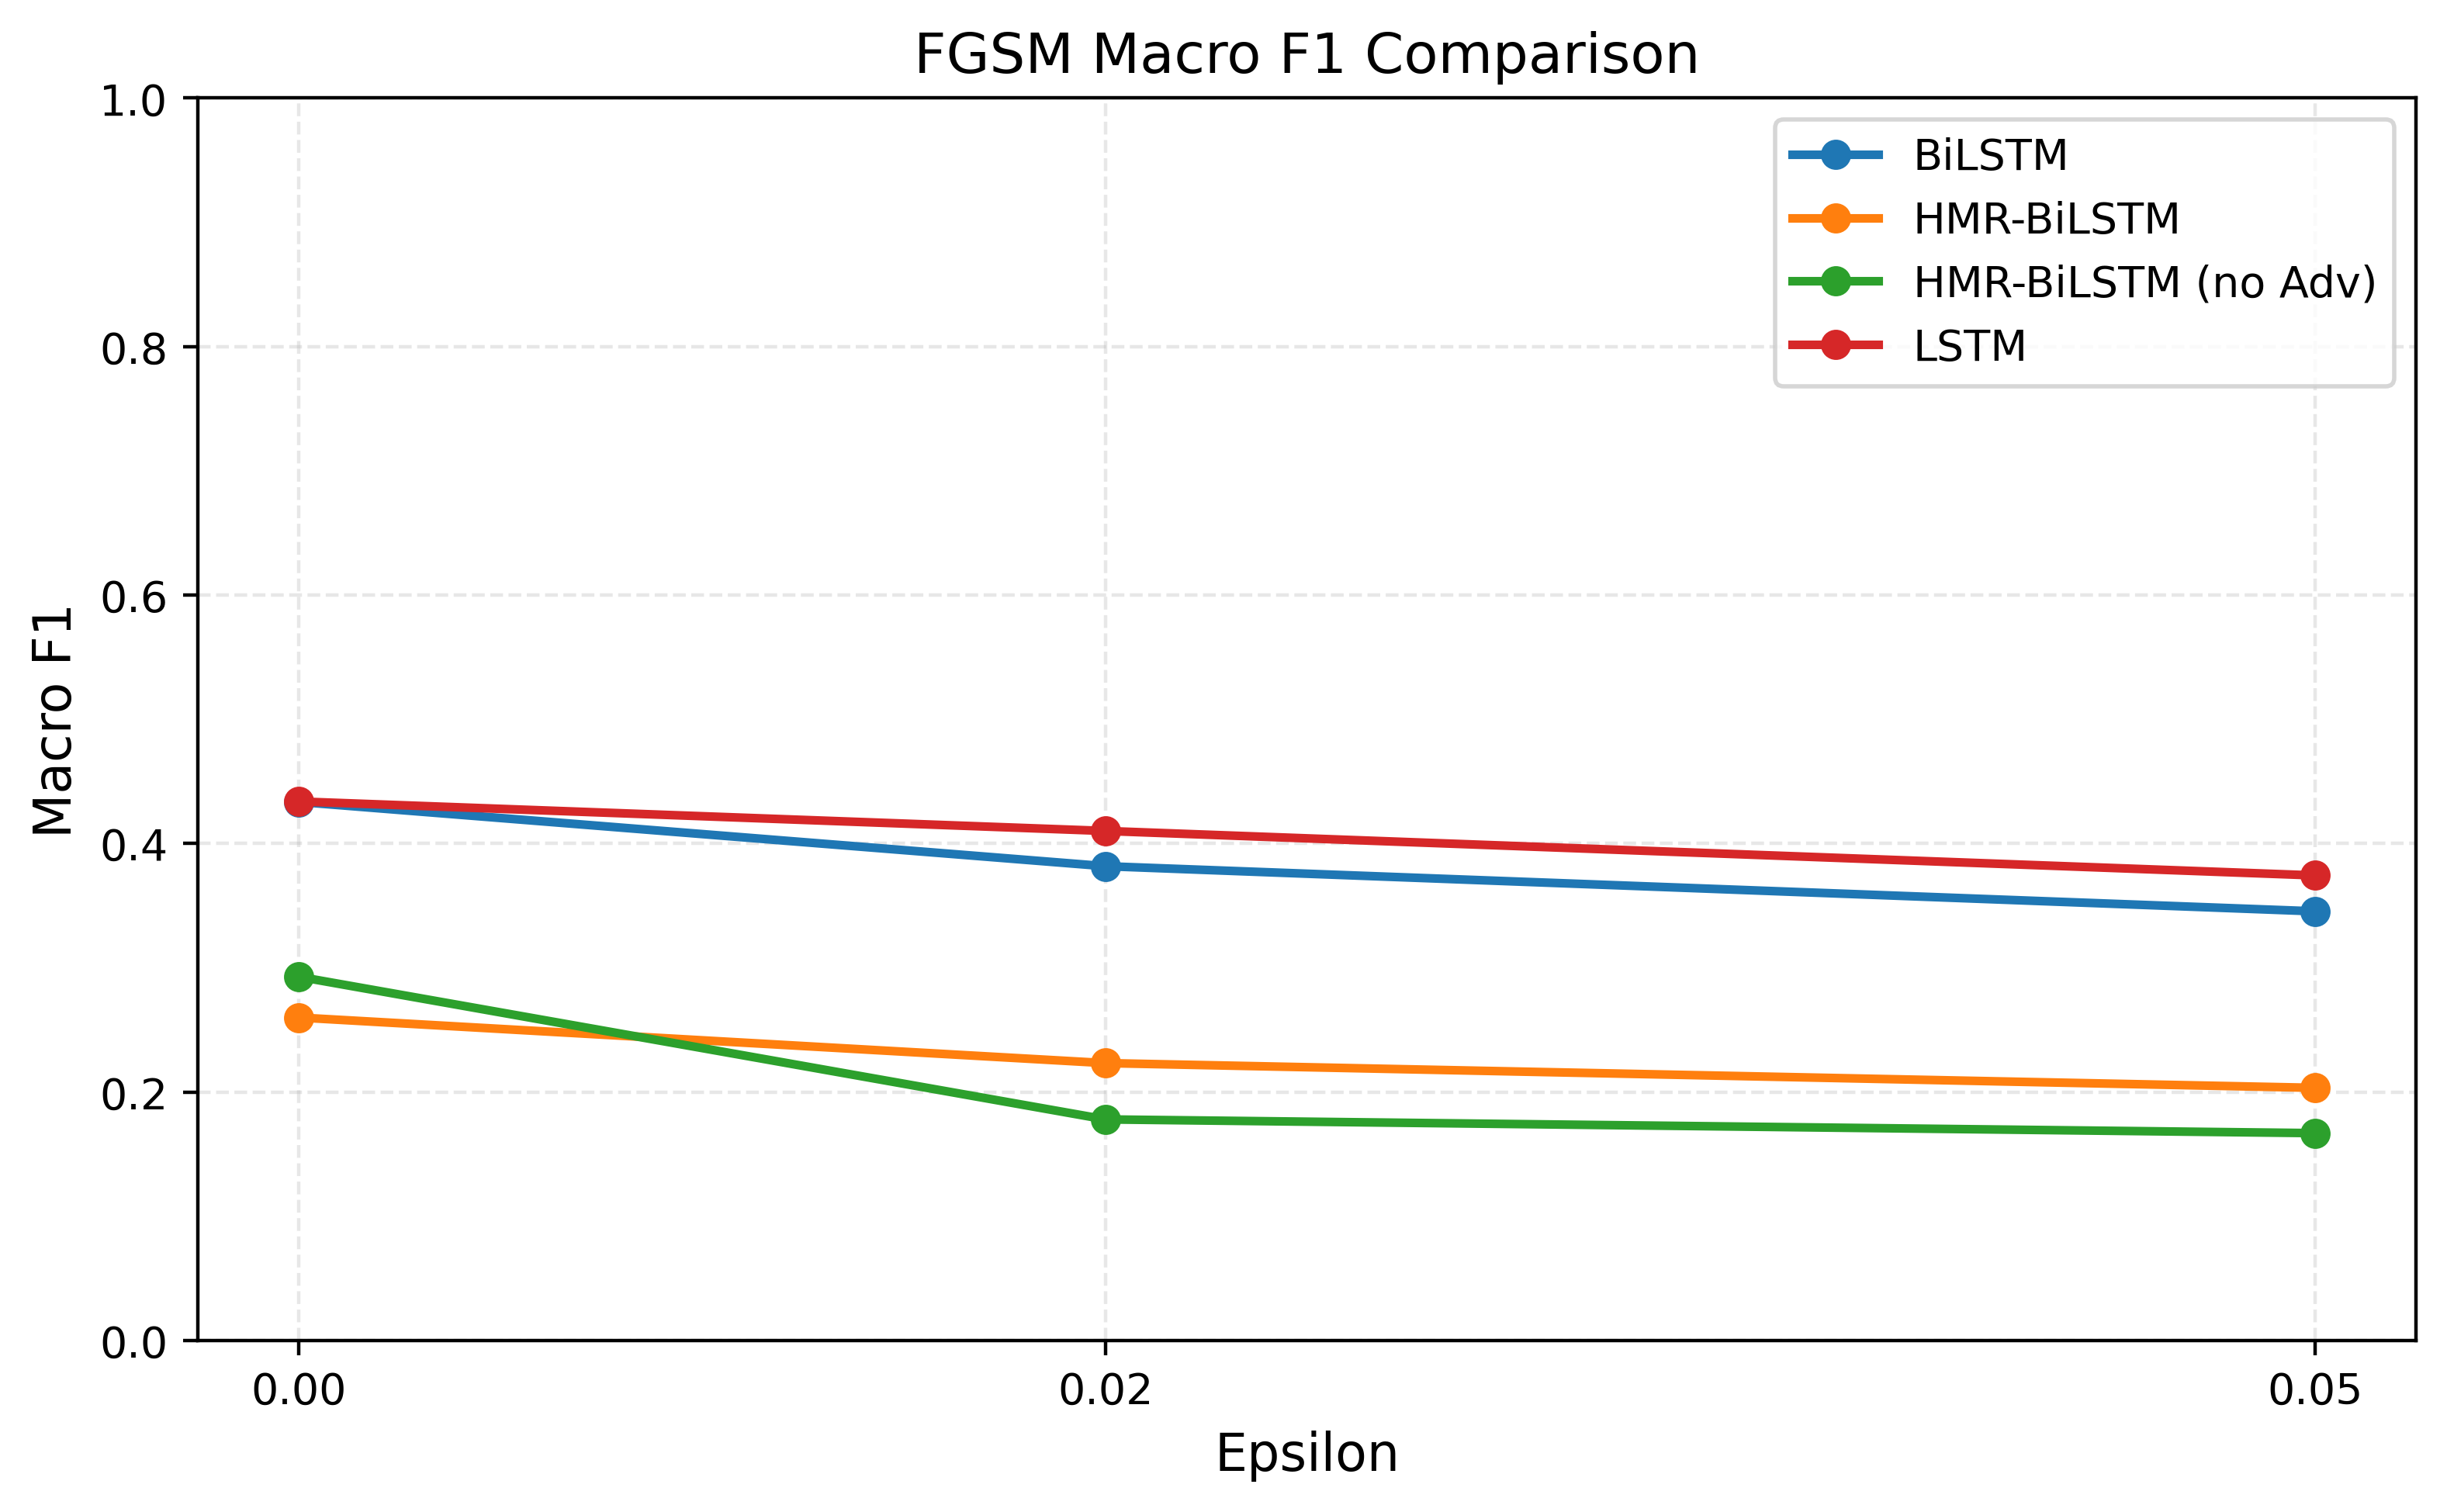
\includegraphics[width=0.75\textwidth]{images/fgsm_baseline_f1_vs_epsilon.png}
\caption{Macro F1 under FGSM attack as a function of the perturbation radius $\varepsilon$, full DS2 test set.}
\label{fig:fgsm_macro}
\end{figure}

\begin{figure}[!t]
\centering
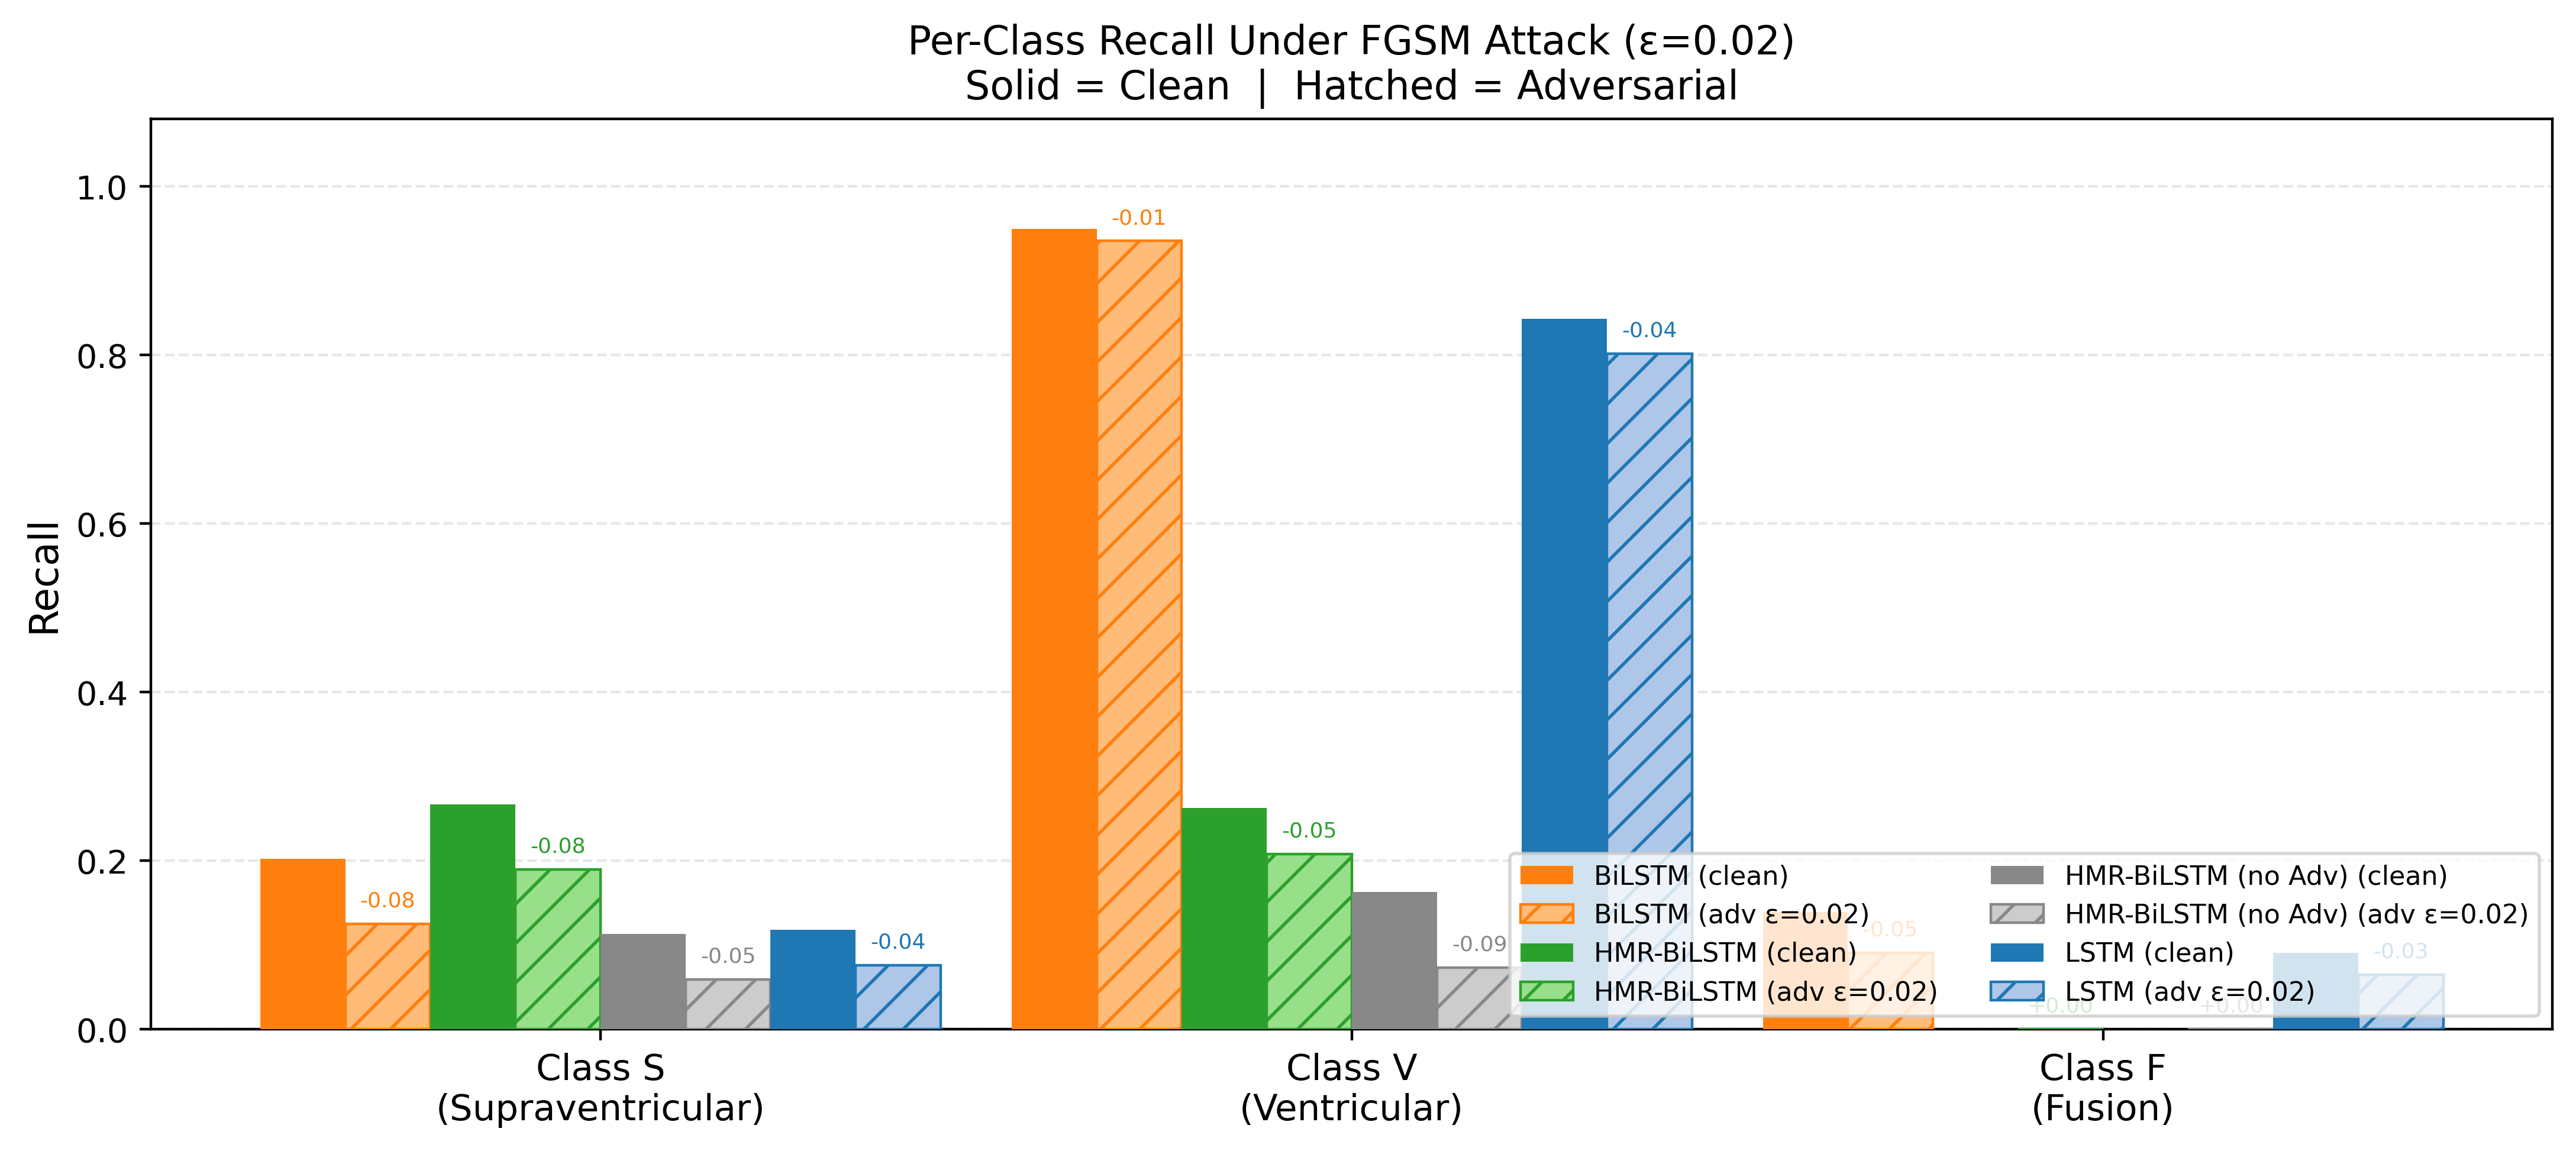
\includegraphics[width=0.75\textwidth]{images/fgsm_per_class_recall_eps0.02.png}
\caption{Per-class recall under FGSM at $\varepsilon = 0.02$, clean vs. adversarial, full DS2 test set.}
\label{fig:fgsm_class}
\end{figure}

\subsection{Noise Robustness}
\begin{table}[htbp]
\caption{Macro F1 under additive Gaussian noise of standard deviation $\sigma$ (clean-trained inputs), full DS2 test set.}
\label{tab:noise}
\centering
\begin{tabular}{@{}lcccccc@{}}
\toprule
\textbf{Model} & $\sigma{=}0$ & $\sigma{=}0.1$ & $\sigma{=}0.2$ & $\sigma{=}0.3$ & $\sigma{=}0.4$ & $\sigma{=}0.5$ \\
\midrule
LSTM & 0.4338 & 0.4426 & 0.4350 & 0.4055 & 0.3365 & 0.2034 \\
BiLSTM & 0.4334 & 0.4103 & 0.3855 & 0.3879 & 0.3973 & \textbf{0.3956} \\
\textbf{HMR-BiLSTM} & \textbf{0.6279} & \textbf{0.6240} & \textbf{0.5417} & \textbf{0.4659} & \textbf{0.4284} & 0.3873 \\
\bottomrule
\end{tabular}
\end{table}

As shown in Table~\ref{tab:noise} and Fig.~\ref{fig:noise_macro}, HMR-BiLSTM keeps the highest macro F1 from $\sigma=0$ through $\sigma=0.4$, but the margin shrinks steadily as noise grows, and at $\sigma=0.5$ BiLSTM edges narrowly ahead (0.3956 vs 0.3873); LSTM, in contrast, collapses sharply beyond $\sigma=0.3$ (down to 0.2034 at $\sigma=0.5$). We read this as HMR-BiLSTM being the more noise-tolerant model across the range that matters for realistic sensor/electrode noise ($\sigma \lesssim 0.3$--0.4 in Z-score units), rather than uniformly dominant at every noise level tested; we do not have a mechanistic explanation for BiLSTM's crossover at the highest noise level and flag it as an observation rather than a designed property.

\begin{figure}[!t]
\centering
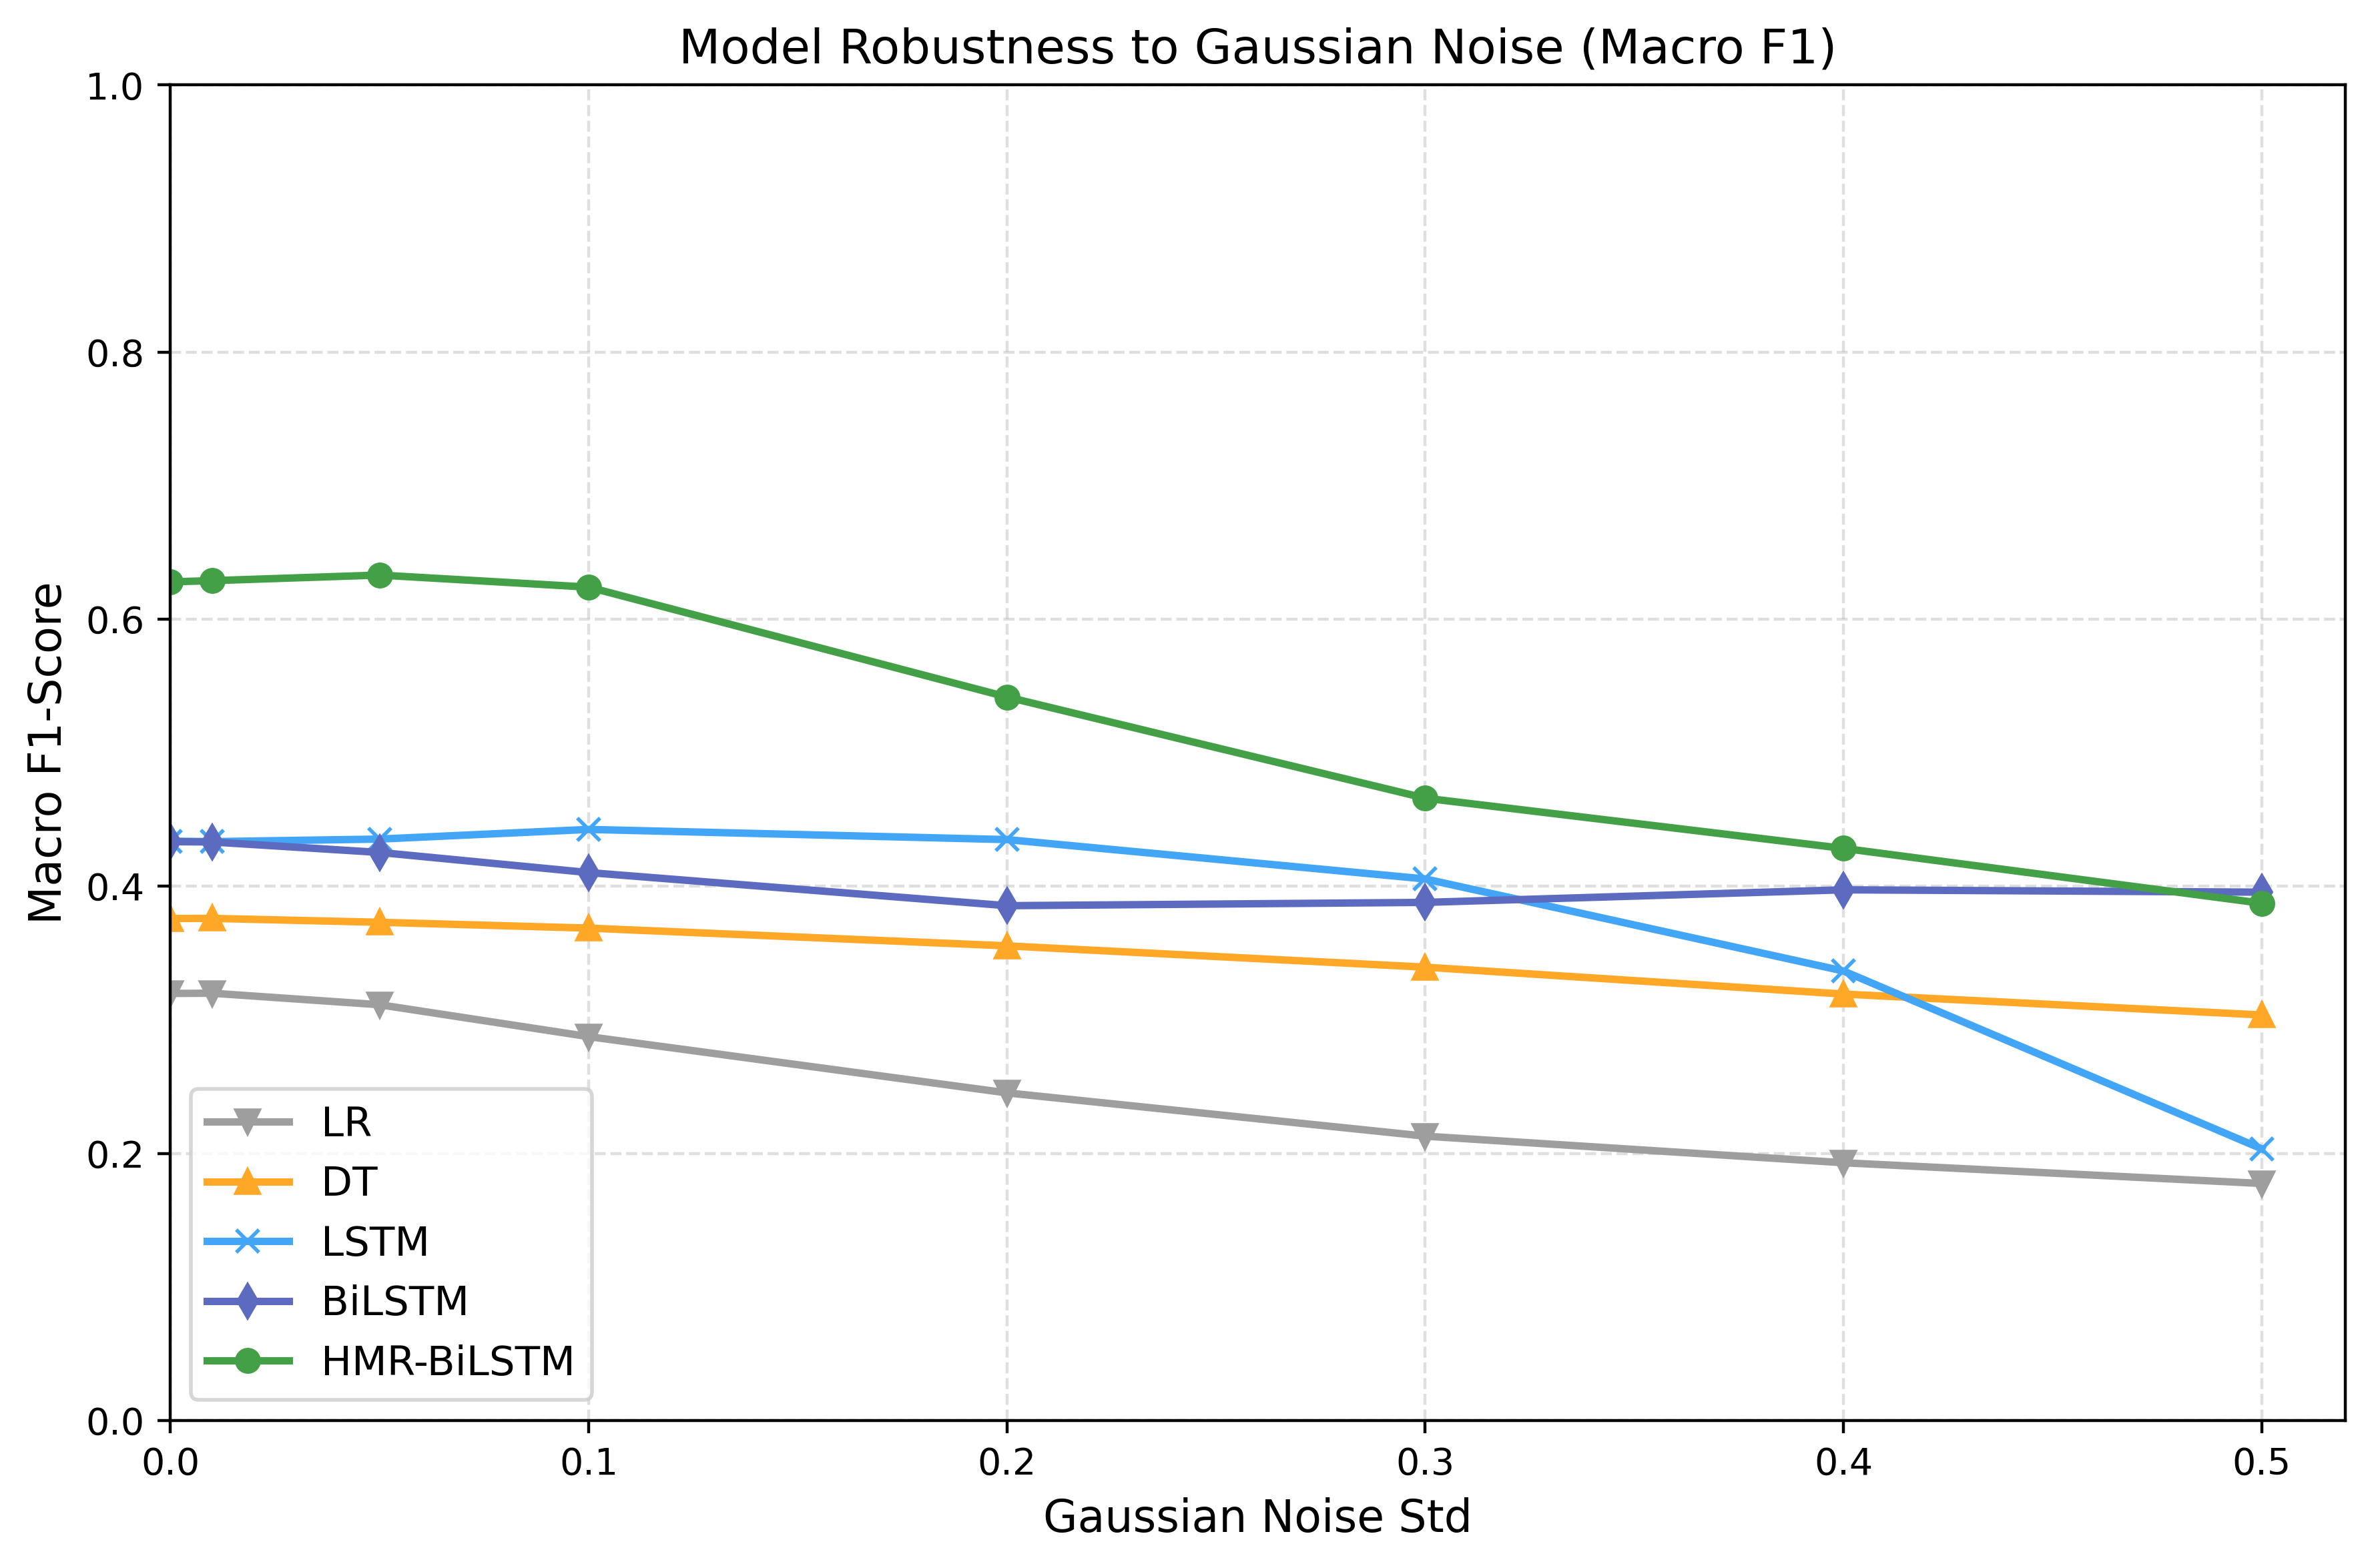
\includegraphics[width=0.8\textwidth]{images/robustness_noise_all.png}
\caption{Macro F1 of five methods as a function of additive Gaussian noise standard deviation $\sigma$, full DS2 test set.}
\label{fig:noise_macro}
\end{figure}

\subsection{Calibration}
\begin{table}[htbp]
\caption{Calibration metrics on the DS2 test set. Lower is better for all four metrics; only HMR-BiLSTM is temperature-scaled (After), since only its checkpoint is used downstream.}
\label{tab:calibration}
\centering
\begin{tabular}{@{}lcccc@{}}
\toprule
\textbf{Model} & \textbf{ECE} & \textbf{Brier} & \textbf{MCE} & \textbf{NLL} \\
\midrule
LSTM & 0.0779 & 0.2461 & 0.2382 & 0.4594 \\
BiLSTM & 0.1078 & 0.2581 & 0.3259 & 0.6311 \\
HMR-BiLSTM (before) & 0.0380 & 0.1075 & 0.4344 & 0.2162 \\
HMR-BiLSTM (after, $T{=}0.929$) & 0.0277 & 0.1057 & 0.6805 & 0.2095 \\
\bottomrule
\end{tabular}
\end{table}

As shown in Table~\ref{tab:calibration} and Fig.~\ref{fig:reliability}, HMR-BiLSTM has the best ECE, Brier score, and NLL of the three models even before temperature scaling, and temperature scaling further improves ECE, Brier, and NLL together (T close to 1 reflects an already fairly well-calibrated model on average). MCE tells a different story: HMR-BiLSTM's worst-case per-bin calibration error is already the highest of the three models before scaling (0.4344) and gets \emph{worse} after temperature scaling (0.6805), meaning a single global temperature that improves average calibration can simultaneously worsen calibration in the model's least-reliable confidence bin. Breaking ECE down by true class exposes where that worst bin lives: conditional ECE (after scaling) is 0.0481 for N and 0.0200 for V, but 0.3362 for S and 0.4027 for F -- both far outside the ``Good'' range that the aggregate ECE of 0.0277 would suggest, and barely changed by temperature scaling (a single scalar cannot fix a class-specific miscalibration). We therefore do not claim HMR-BiLSTM is well-calibrated on its two hardest classes; aggregate ECE here is dominated by the majority Normal class, and a clinician reading only the headline ECE would be misled about the trustworthiness of the model's S/F predictions specifically.

\begin{figure}[!t]
\centering
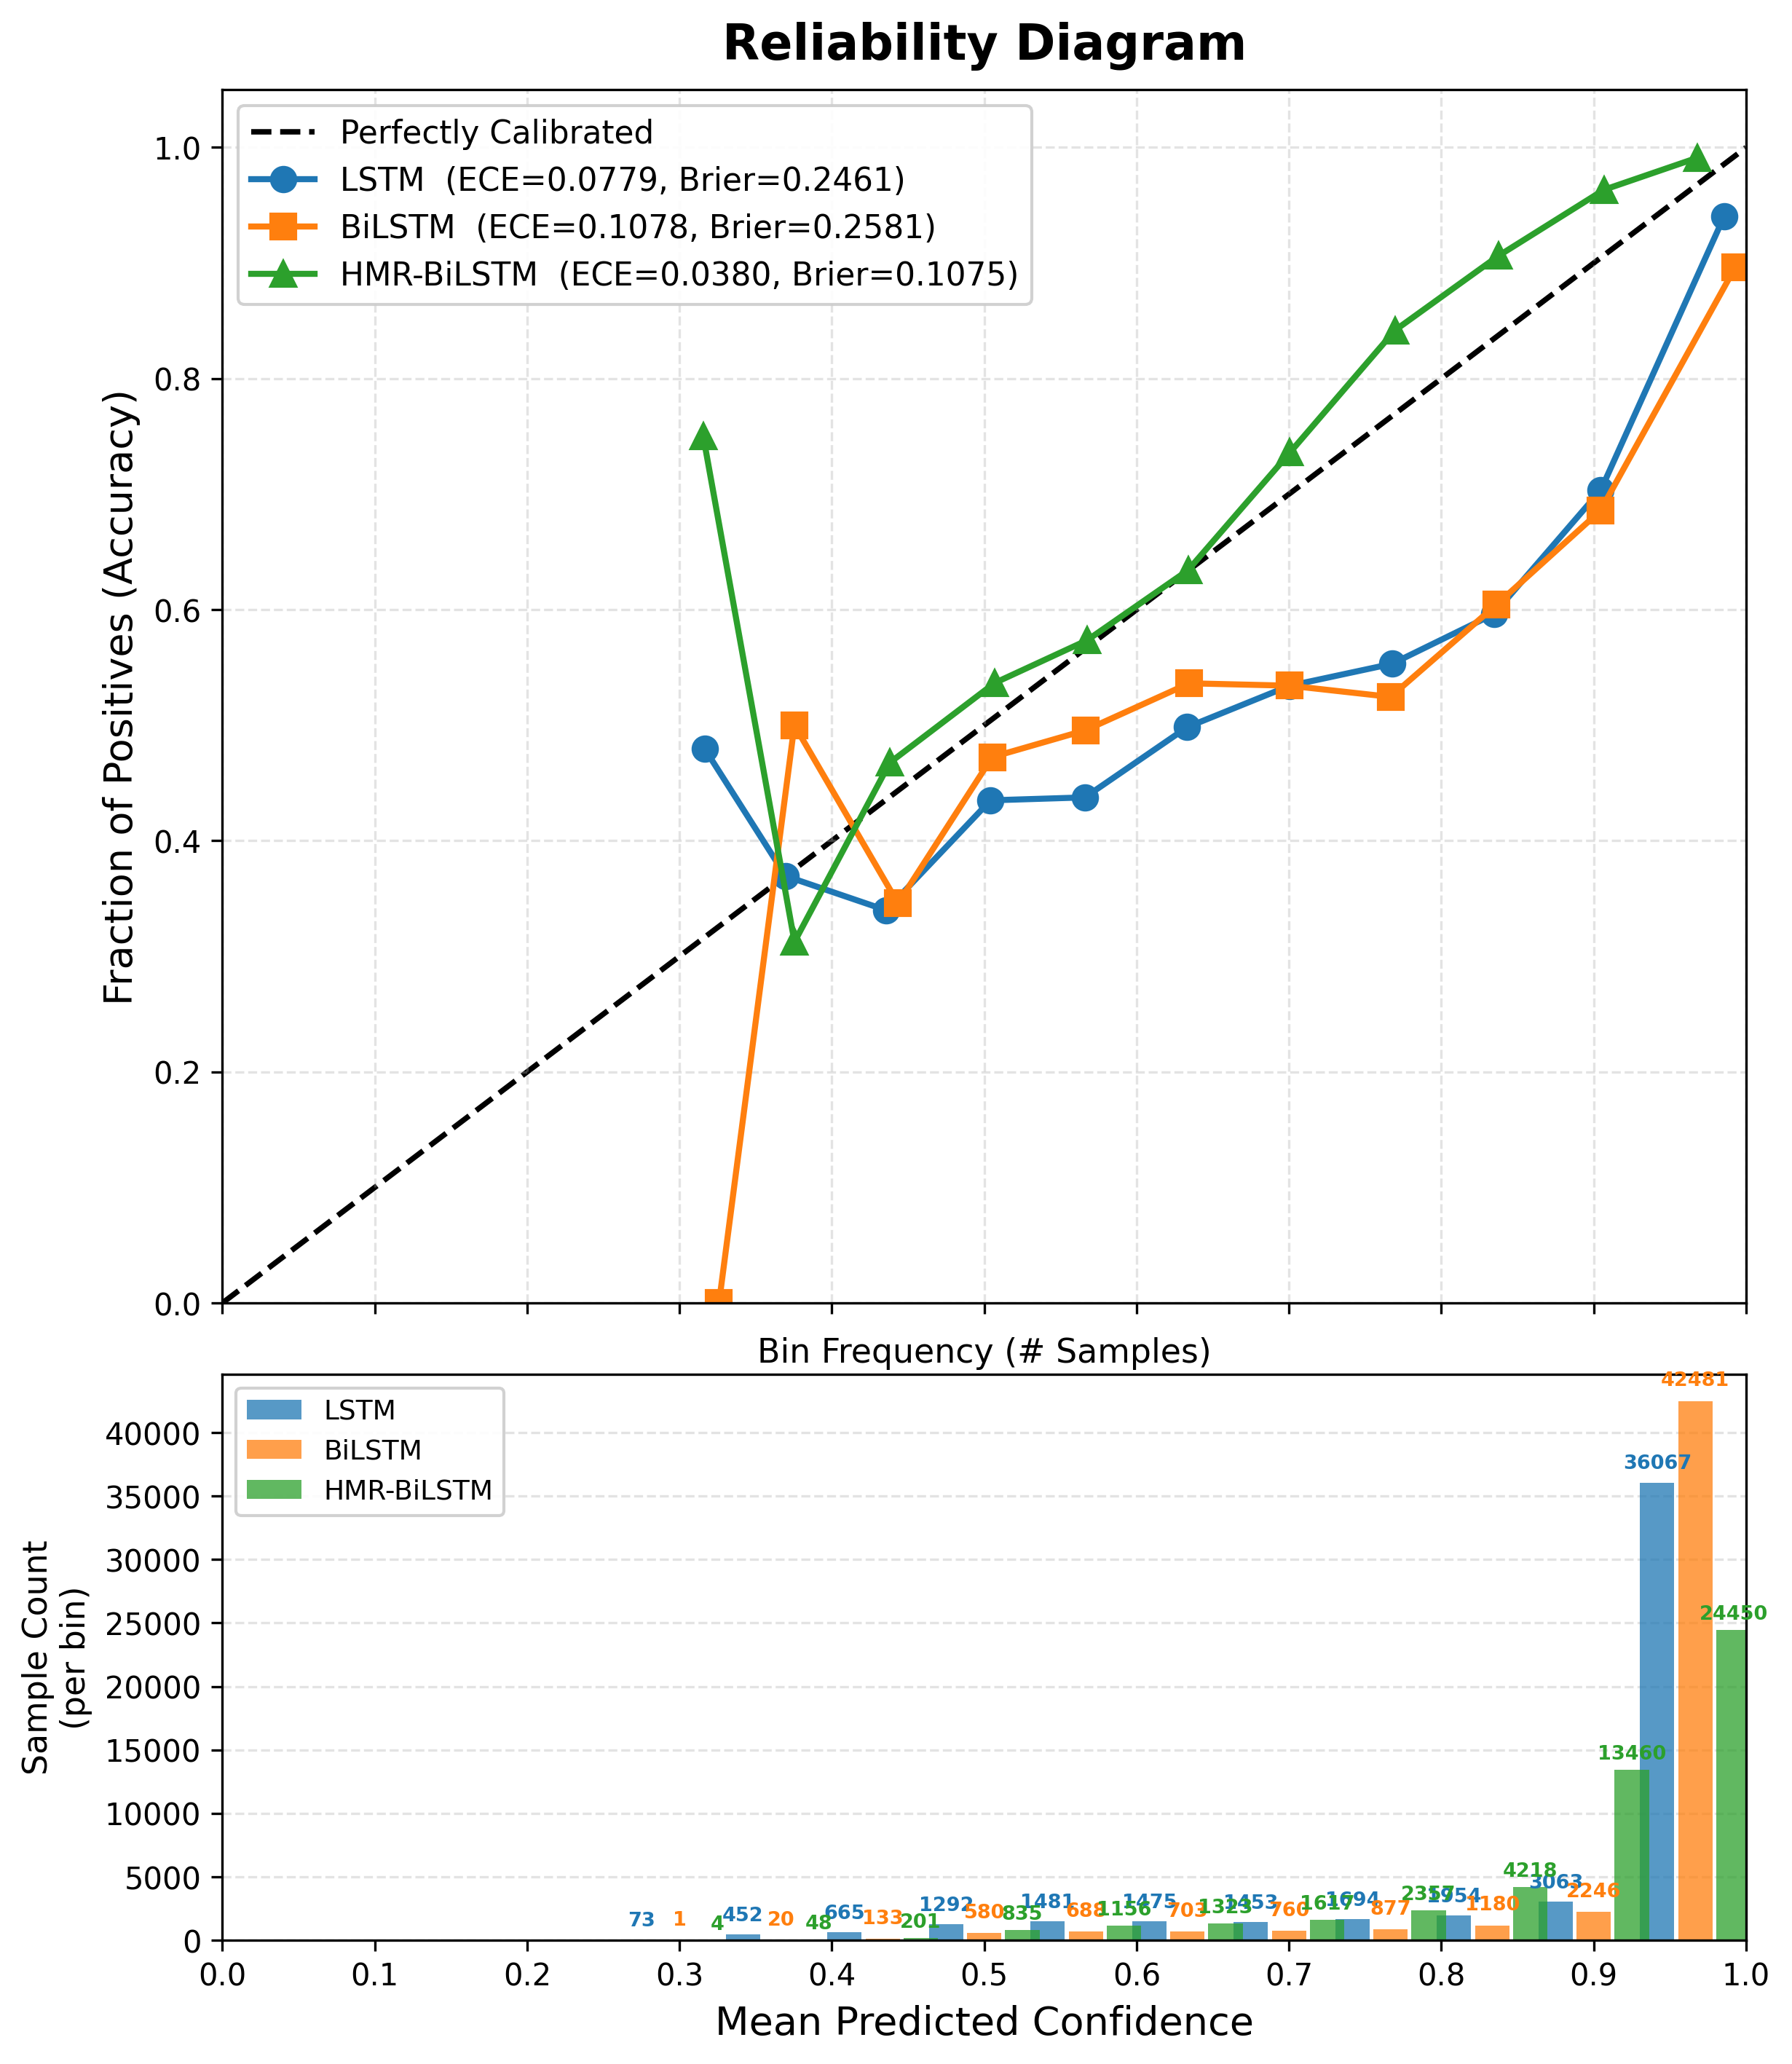
\includegraphics[width=0.7\textwidth]{images/reliability_diagram.png}
\caption{Reliability diagram (confidence vs. accuracy, top; bin sample counts, bottom) for LSTM, BiLSTM, and HMR-BiLSTM on the DS2 test set.}
\label{fig:reliability}
\end{figure}

\subsection{Uncertainty Quantification}
We estimate predictive uncertainty with MC-Dropout (50 stochastic forward passes) and a 3-member Deep Ensemble (independently initialised and trained checkpoints), both applied to the HMR-BiLSTM checkpoint used above. Mean predictive entropy by true class is consistent across both methods: Normal $0.379$/$0.421$ (MC-Dropout/Ensemble), Supraventricular $0.567$/$0.619$, Ventricular $0.269$/$0.323$ (lowest), and Fusion $0.926$/$0.946$ (highest, roughly $3\times$ the Ventricular value under either method). This cross-method agreement is, we think, a more meaningful trustworthiness signal than the single-pass calibration numbers in Section 5.5: even though HMR-BiLSTM's point predictions on Fusion beats are unreliable (F1 0.296 on the full test set, Section 5.1), both independent uncertainty-estimation methods correctly flag Fusion predictions as the least confident of any class, which supports using predictive entropy as a triage signal (route high-entropy predictions to a clinician) rather than relying on the model's raw softmax confidence, which Section 5.5 shows is miscalibrated specifically on this class. Out-of-distribution detection (synthetic corruption: Gaussian noise, baseline wander, random crop, signal shift) is comparatively weak under both methods, with AUROC of 0.610 (MC-Dropout) and 0.604 (Ensemble) -- only modestly above chance -- which we report as a limitation rather than a strength.

\subsection{Interpretability Analysis}
The attention pooling weights $\gamma_t$ can be overlaid on the raw waveform to show which time steps drove a given decision, and the residual gate $r_t$ (Fig.~\ref{fig:gates}) can be tracked per class across the recurrent loop. For each of the four AAMI classes we selected the highest-confidence \emph{correctly classified} DS2 test beat (N: conf.\ 0.9871; S: 0.9732; V: 0.9955; F: 0.8537 -- notably lower than the other three, consistent with Fusion being the hardest class throughout this paper) and overlaid $\gamma_t$ on the raw trace with estimated P/QRS/T regions (Fig.~\ref{fig:case_normal}, Fig.~\ref{fig:case_svf}, Fig.~\ref{fig:case_v}, Fig.~\ref{fig:case_f}).

Qualitatively, attention concentrates near the R-peak/QRS complex for all four cases, with the Supraventricular and Fusion examples showing a visibly wider spread of attention mass either side of the peak than the sharply localised Normal and Ventricular examples -- consistent with the model needing a longer window of context to resolve these harder classes, even on beats it ultimately classifies correctly and confidently. We treat this as a directional, single-example observation rather than a class-level statistical claim; our own SHAP-based feature-importance check (Integrated-Gradients-consistency validated) found the \emph{aggregate}, dataset-wide top-10 most important time steps clustered tightly around the R-peak region (samples 88--96 of 187) for all five classes, including Supraventricular, rather than the clearly separated per-class regions (e.g.\ a distinct P-wave-only focus for S) we had anticipated from the single-example attention overlays. We view this attention-vs-SHAP disagreement as an honest negative/mixed interpretability finding worth reporting rather than smoothing over: the two explanation methods do not obviously agree on \emph{where} the model's evidence lives at the population level, even when a single example's attention plot looks clinically plausible, and reconciling the two -- together with a proper clinician validation study -- is left for future work.

\begin{figure}[!t]
\centering
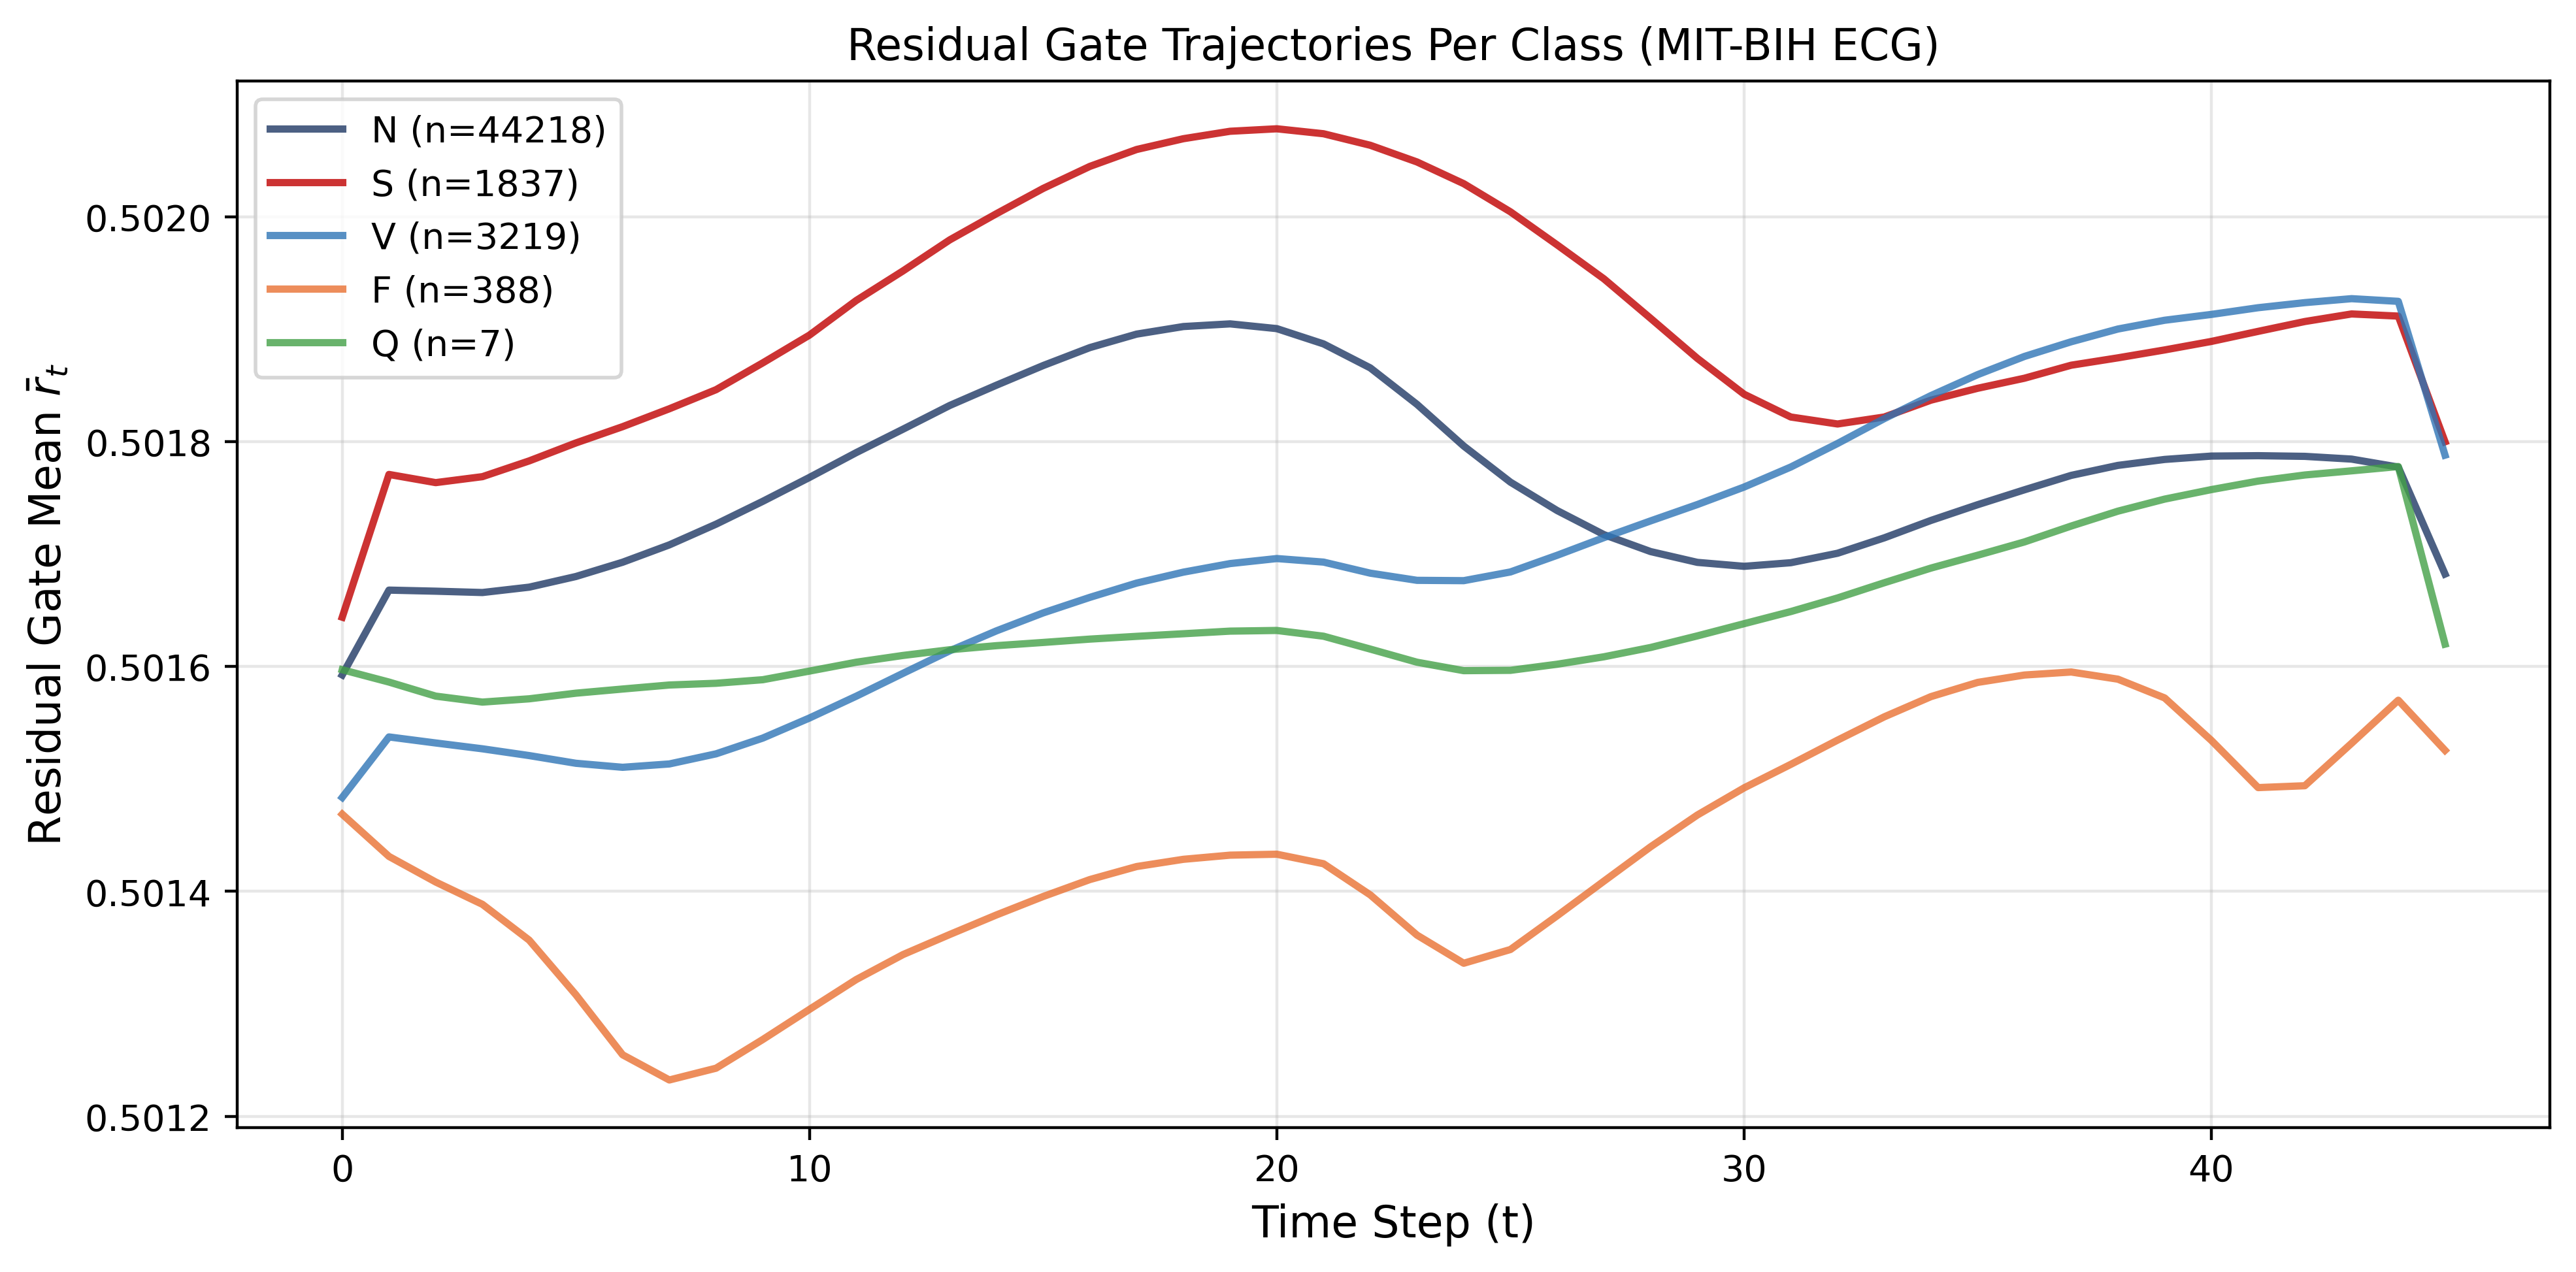
\includegraphics[width=0.8\textwidth]{images/gate_trajectories.png}
\caption{Mean residual gate $r_t$ trajectory per class over the recurrent time steps, DS2 test set.}
\label{fig:gates}
\end{figure}

\begin{figure}[!t]
\centering
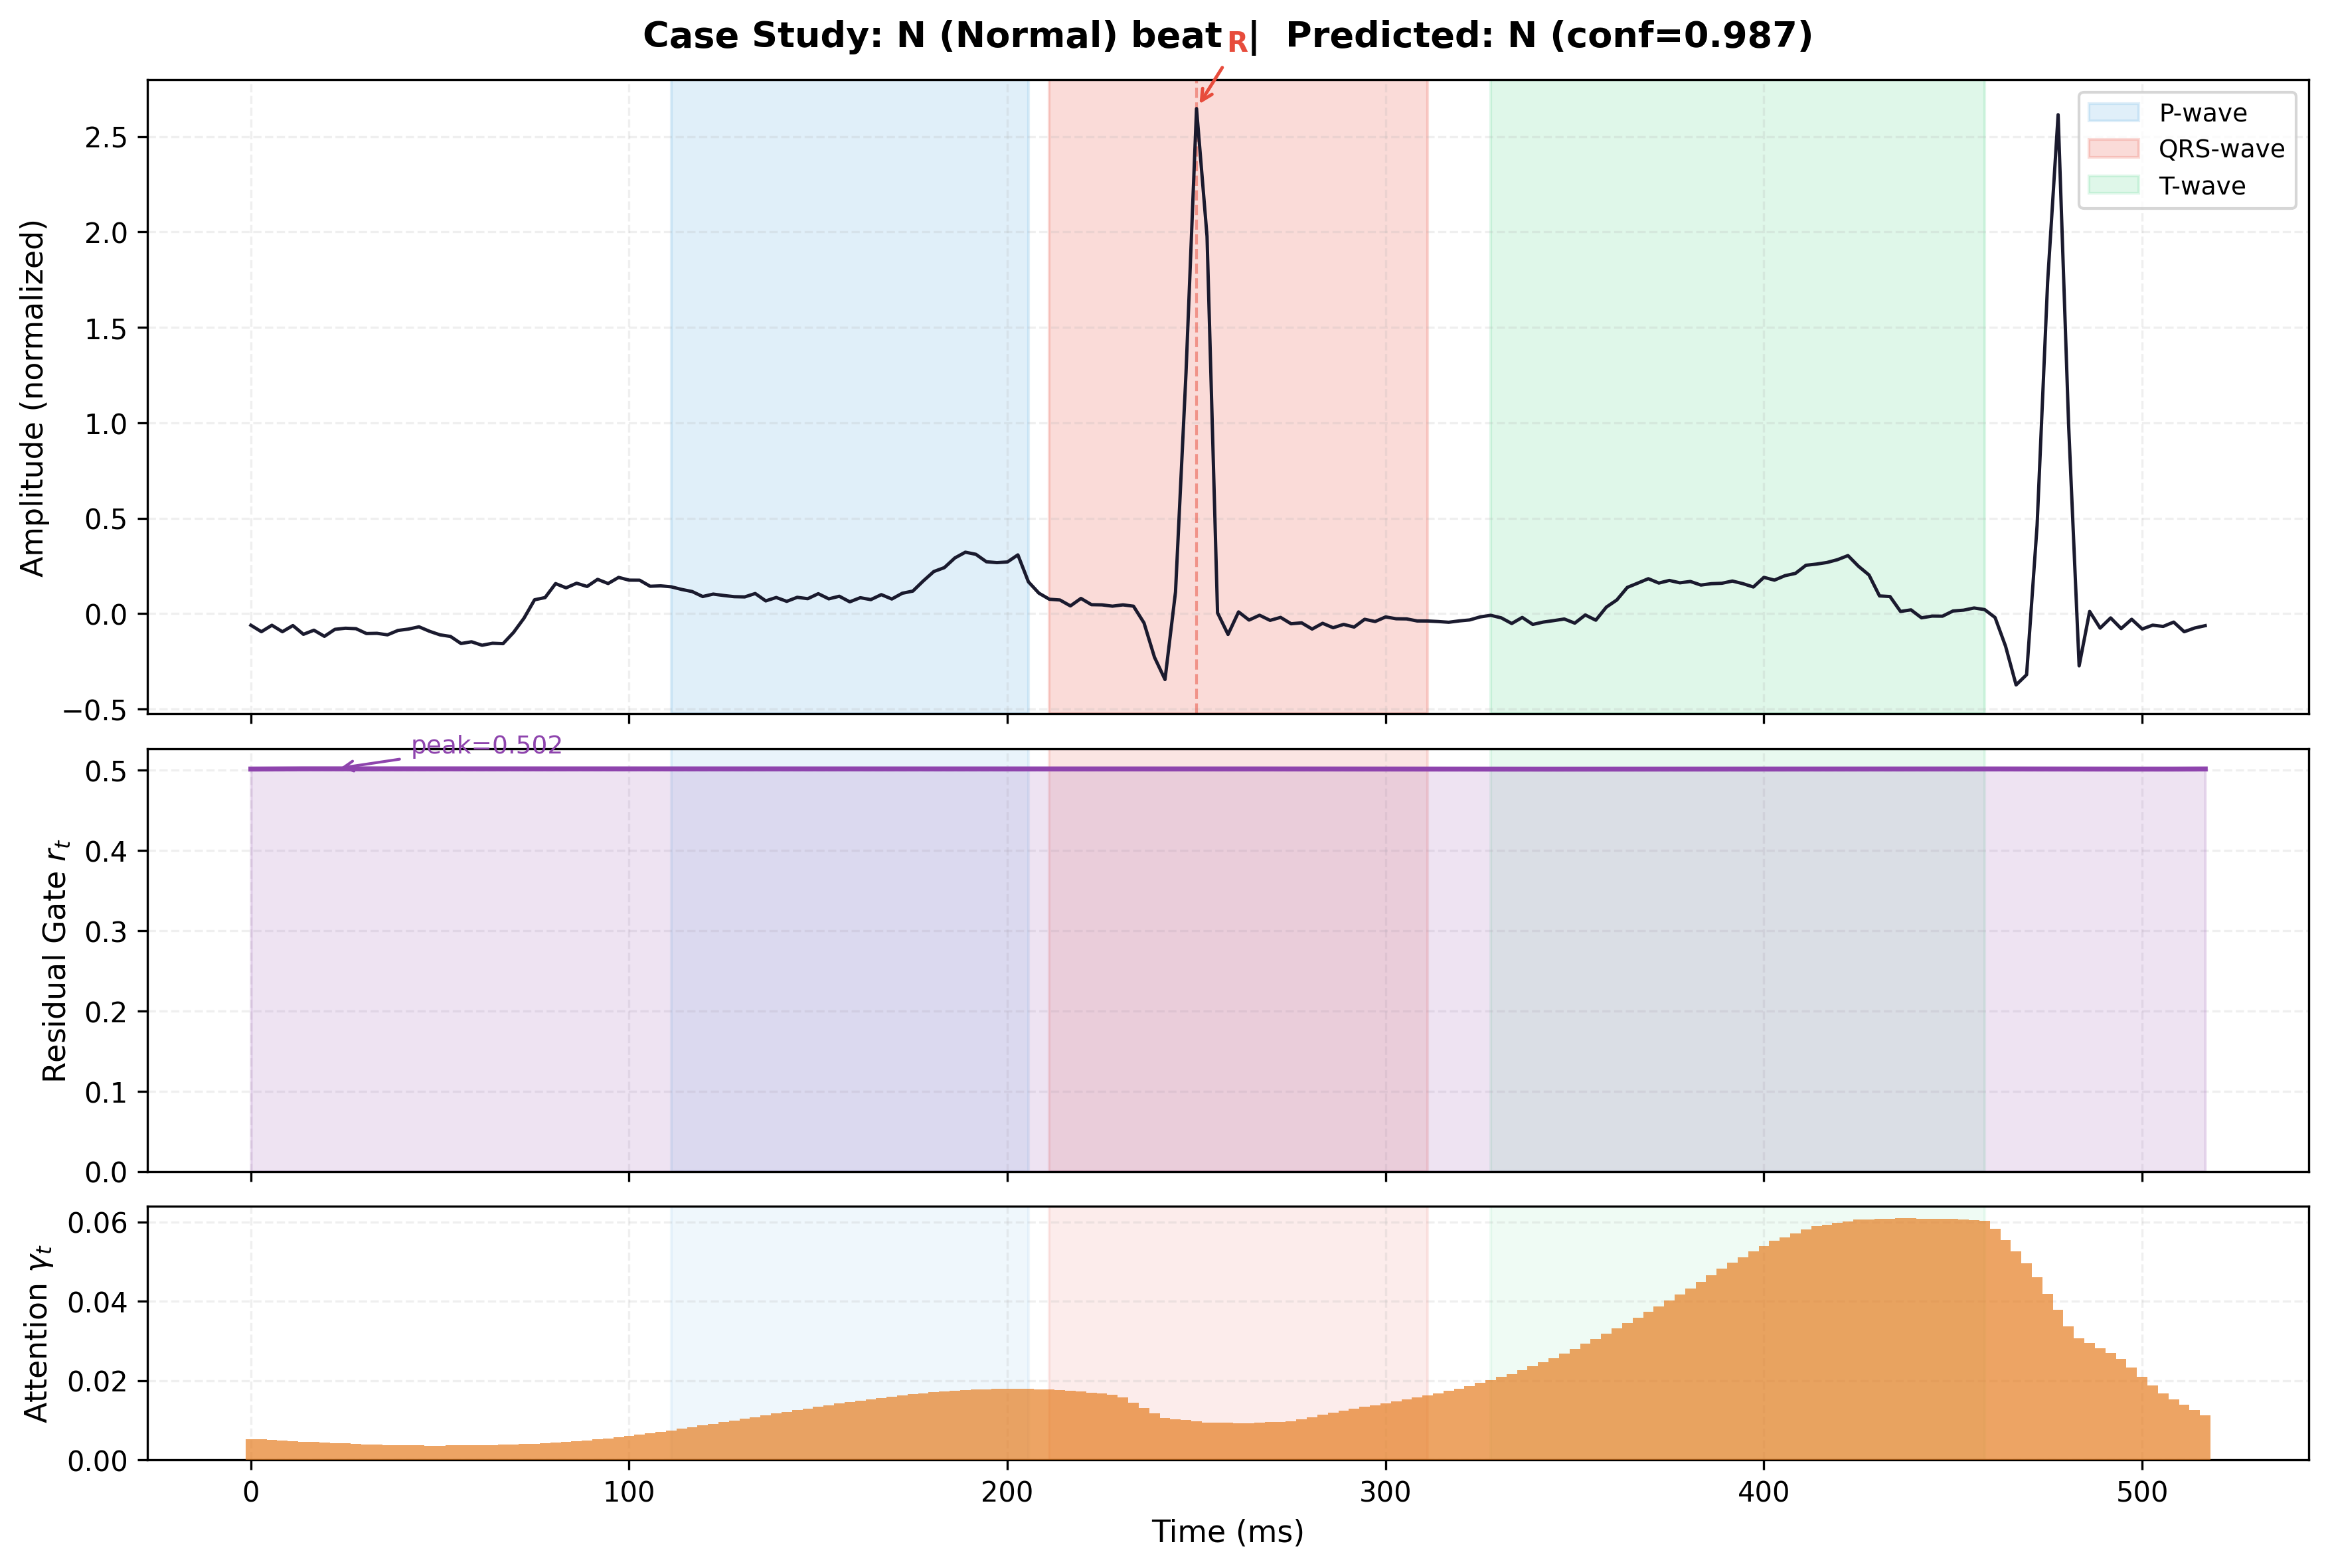
\includegraphics[width=0.75\textwidth]{images/case_normal.png}
\caption{Case study, Normal beat (confidence 0.9871): raw ECG waveform, estimated P/QRS/T regions, and attention pooling weights $\gamma_t$ on a shared time axis.}
\label{fig:case_normal}
\end{figure}

\begin{figure}[!t]
\centering
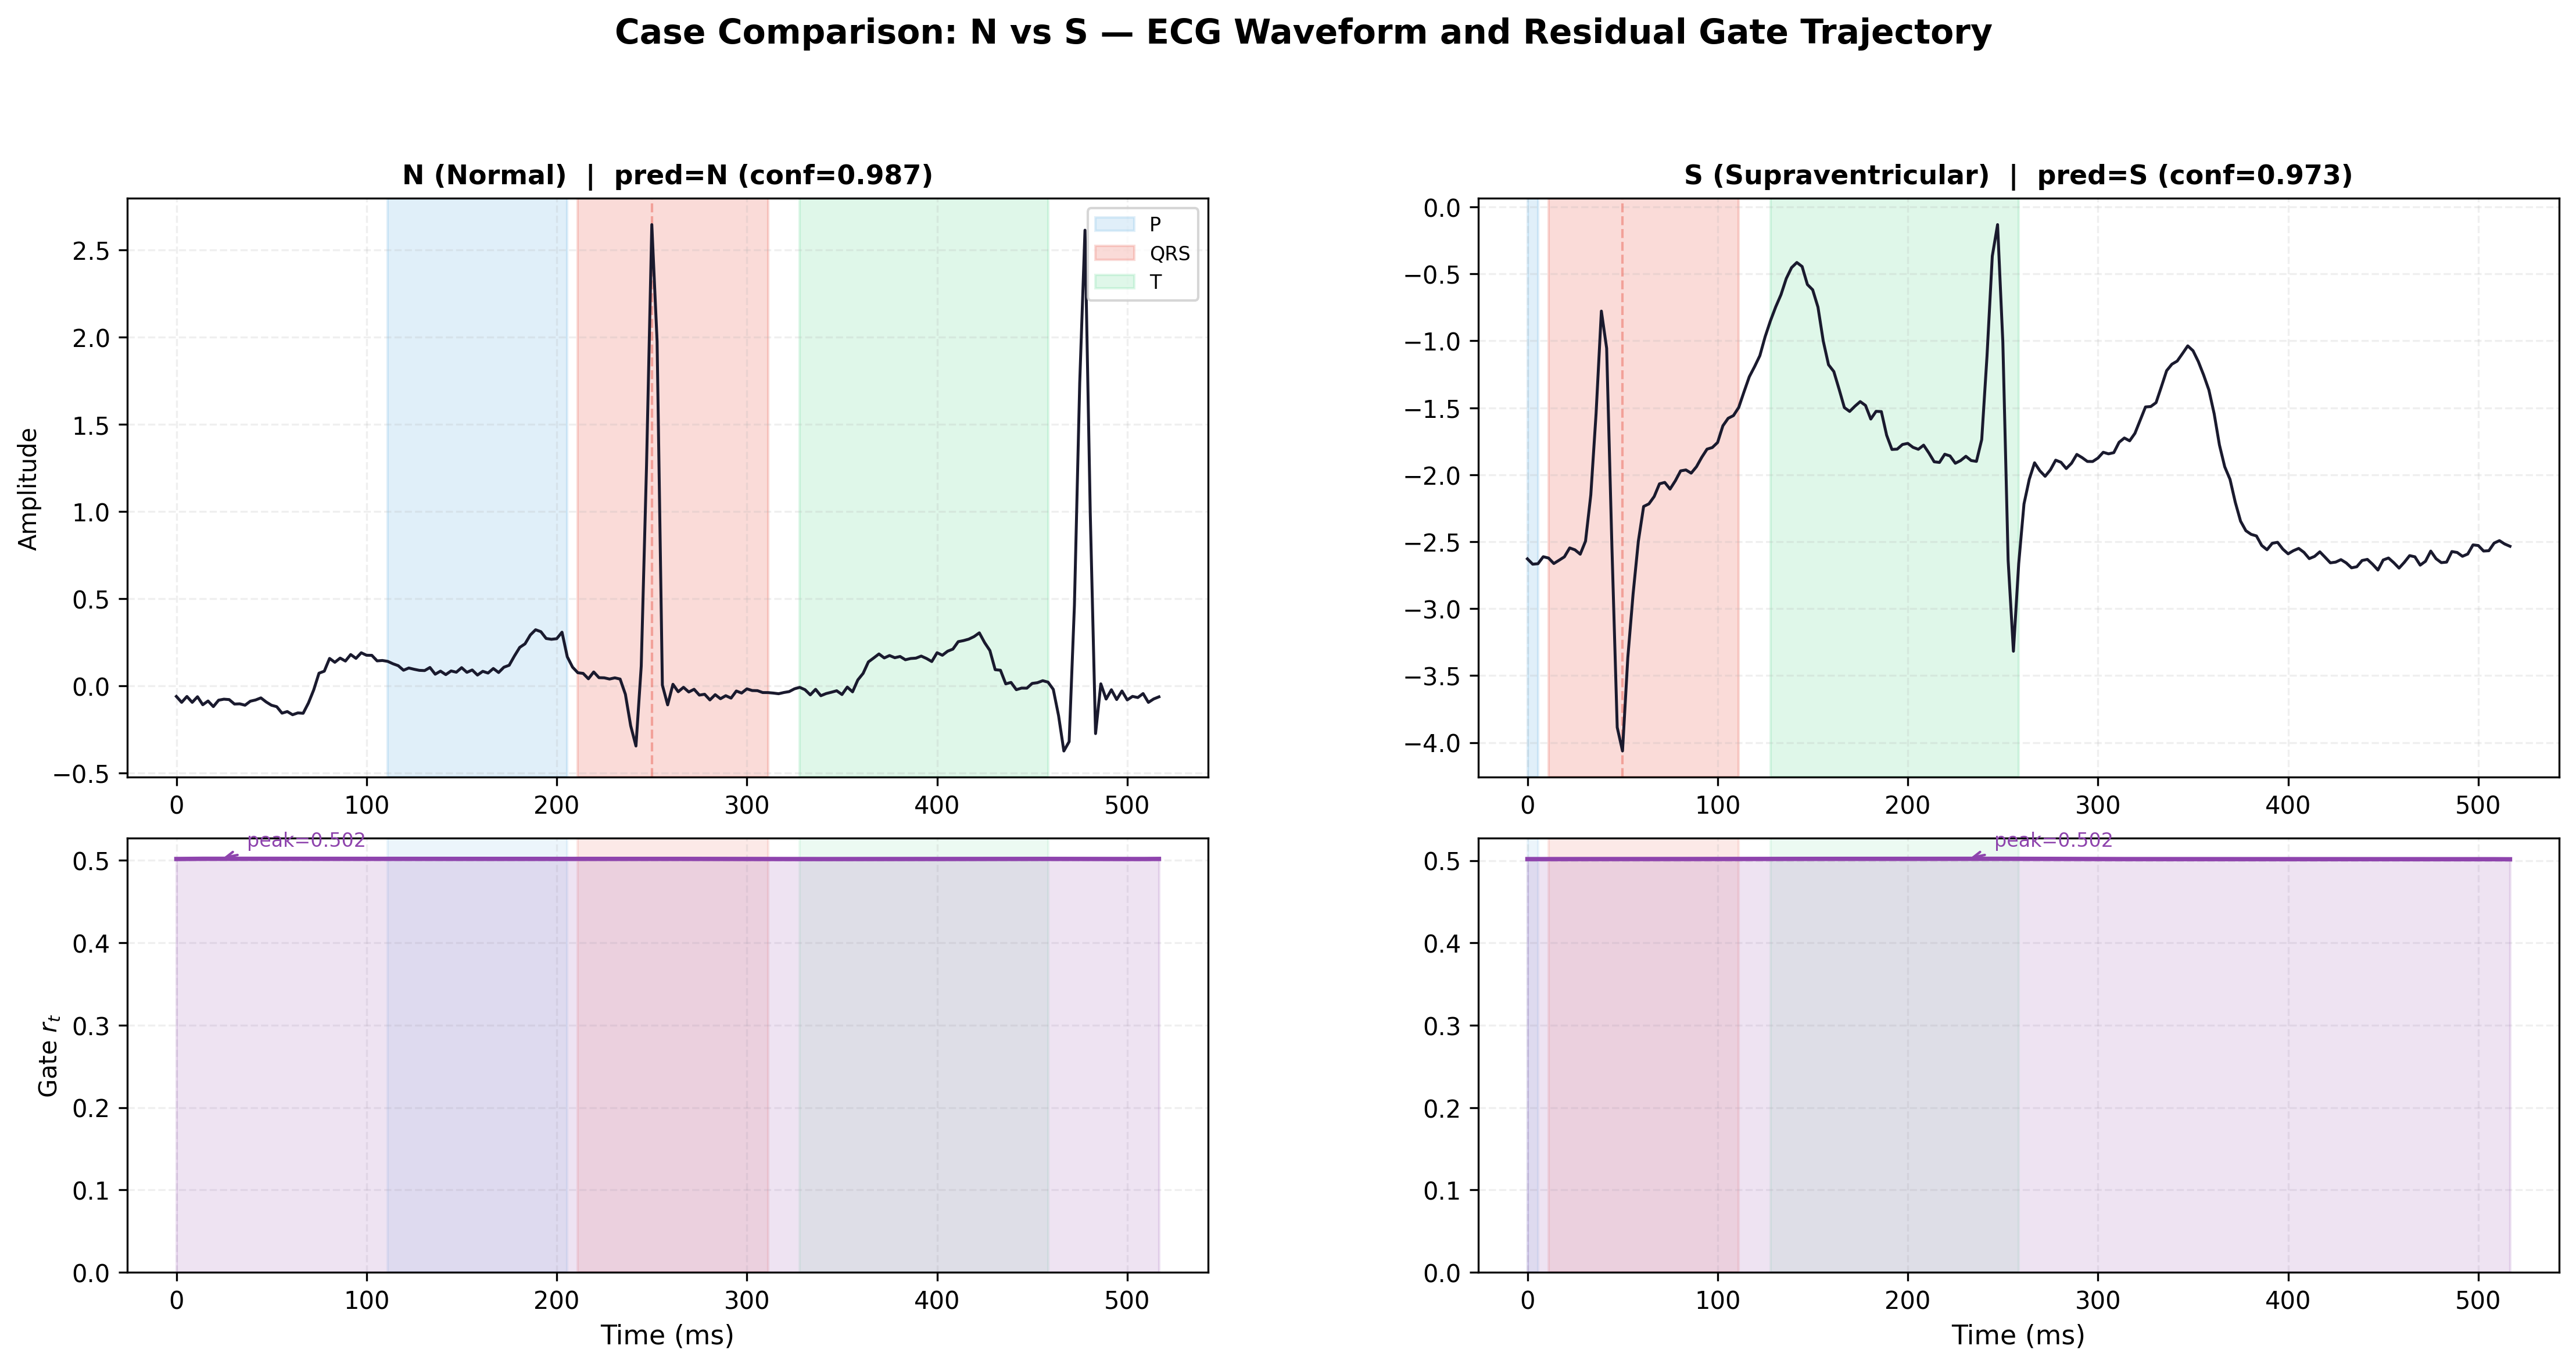
\includegraphics[width=0.8\textwidth]{images/case_comparison_N_vs_S.png}
\caption{Normal vs. Supraventricular case comparison (S confidence 0.9732): raw waveform, estimated P/QRS/T regions, and $\gamma_t$ for both beats on a shared time axis.}
\label{fig:case_svf}
\end{figure}

\begin{figure}[!t]
\centering
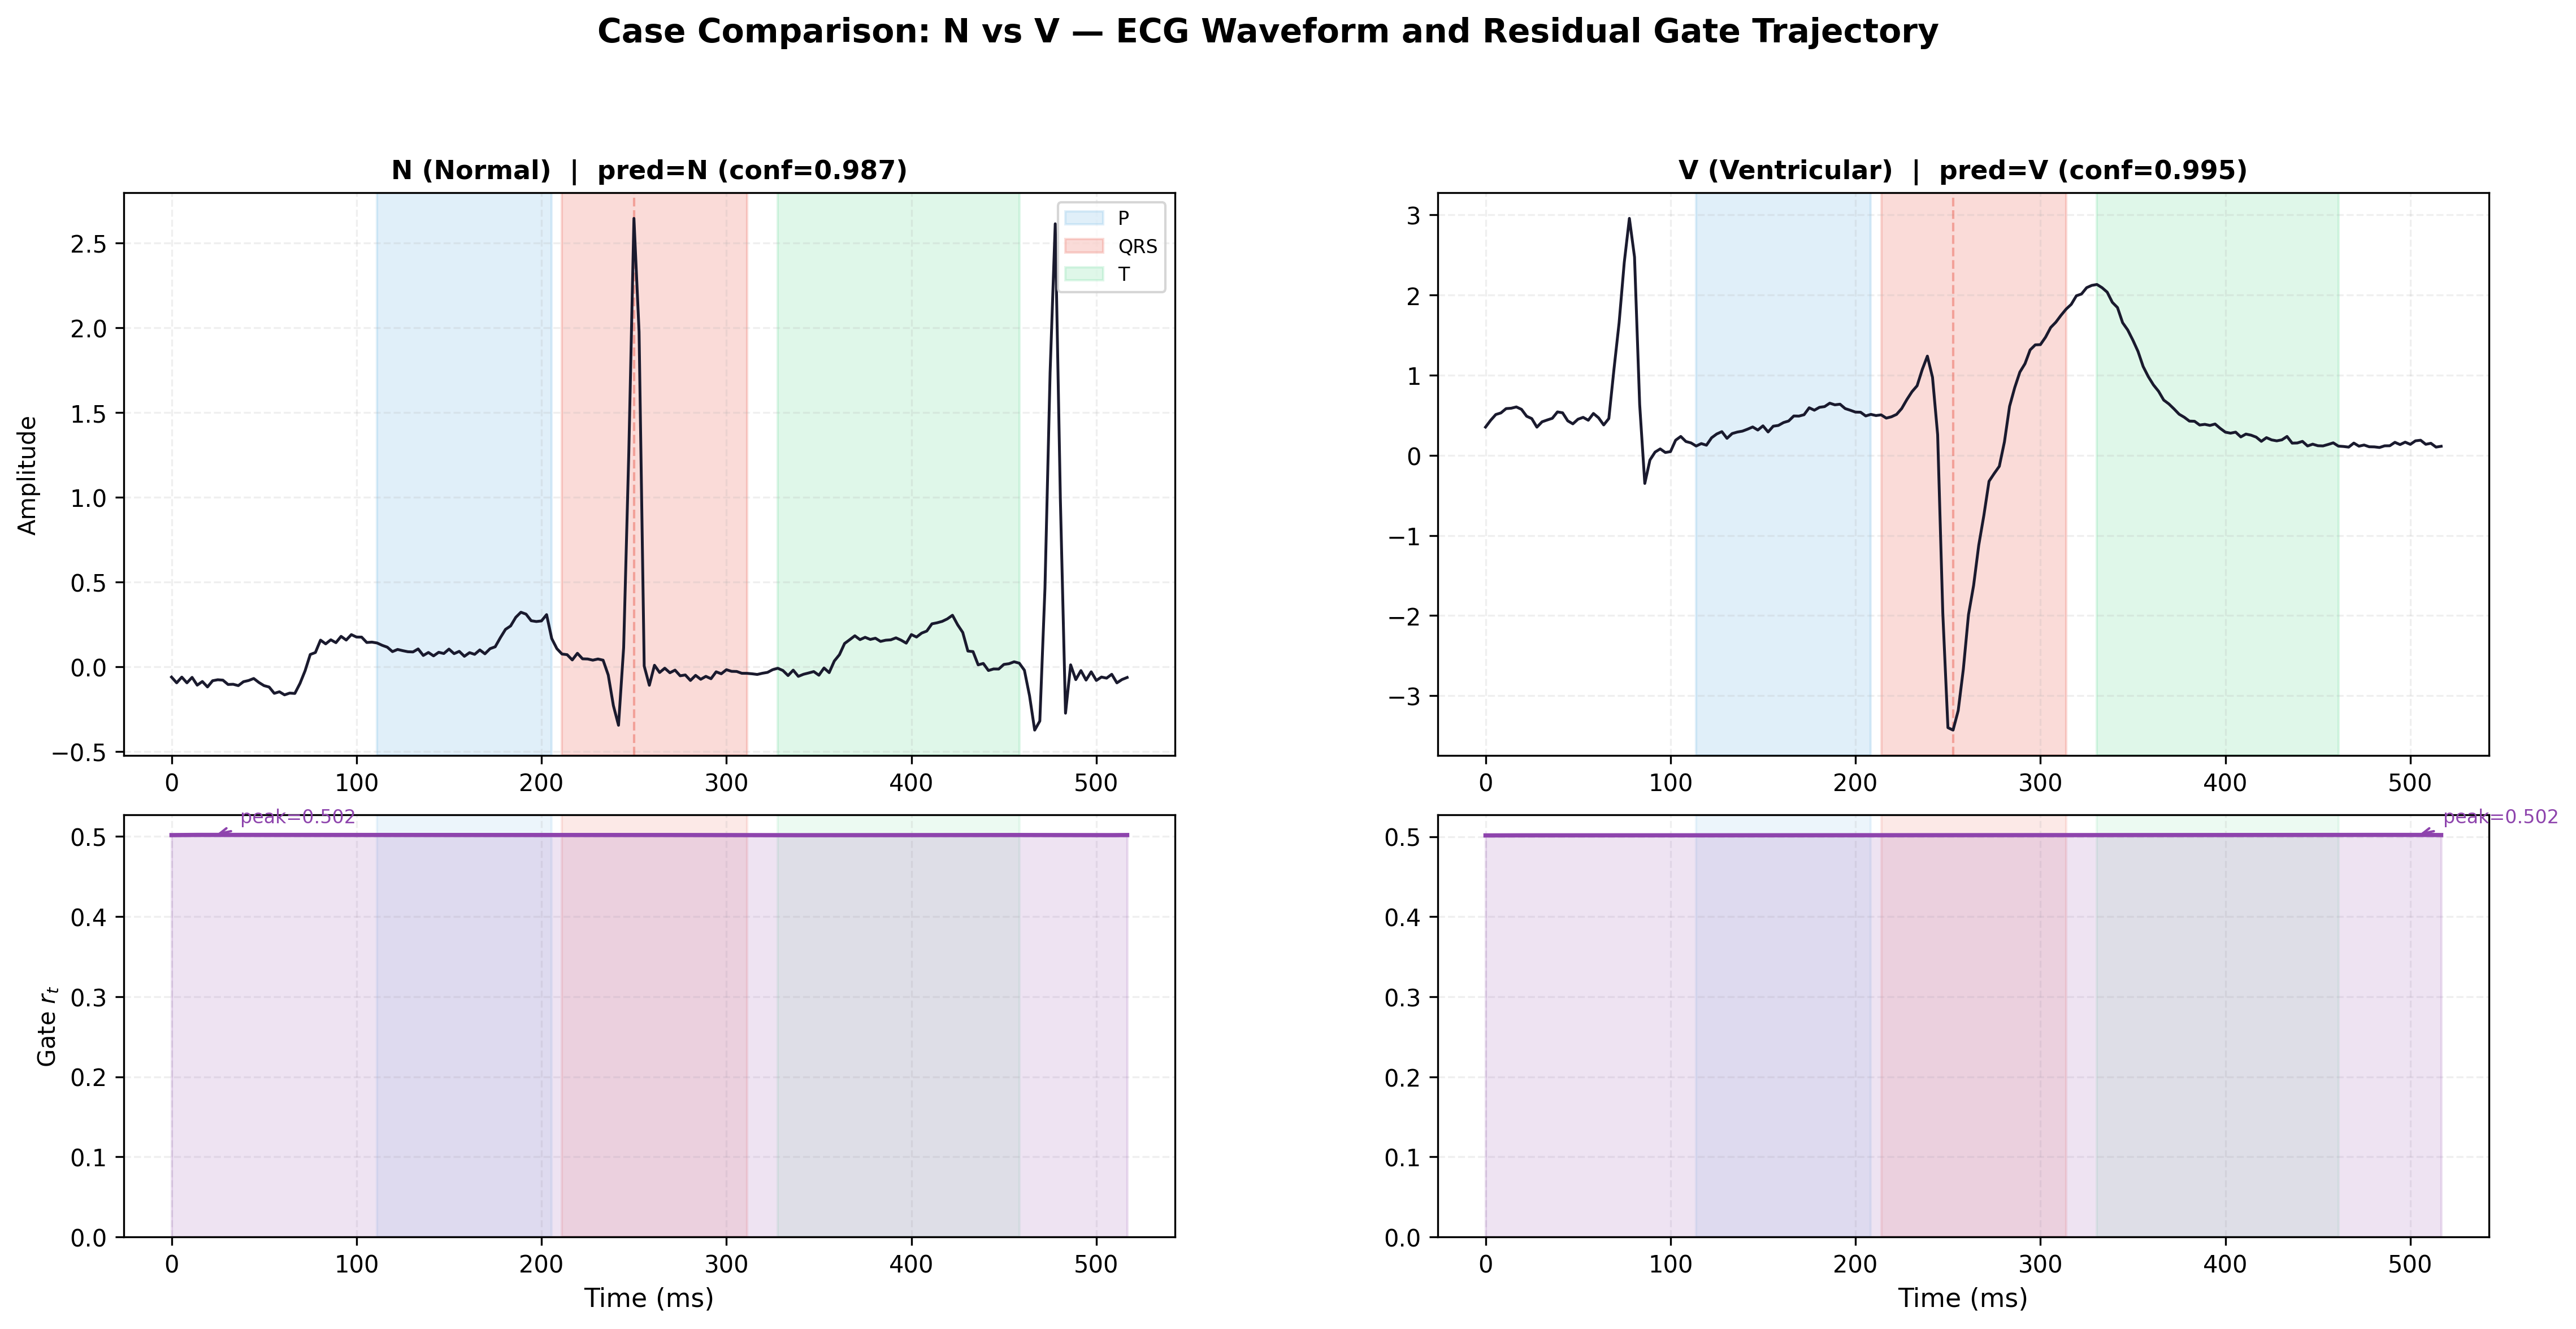
\includegraphics[width=0.8\textwidth]{images/case_comparison_N_vs_V.png}
\caption{Normal vs. Ventricular case comparison (V confidence 0.9955).}
\label{fig:case_v}
\end{figure}

\begin{figure}[!t]
\centering
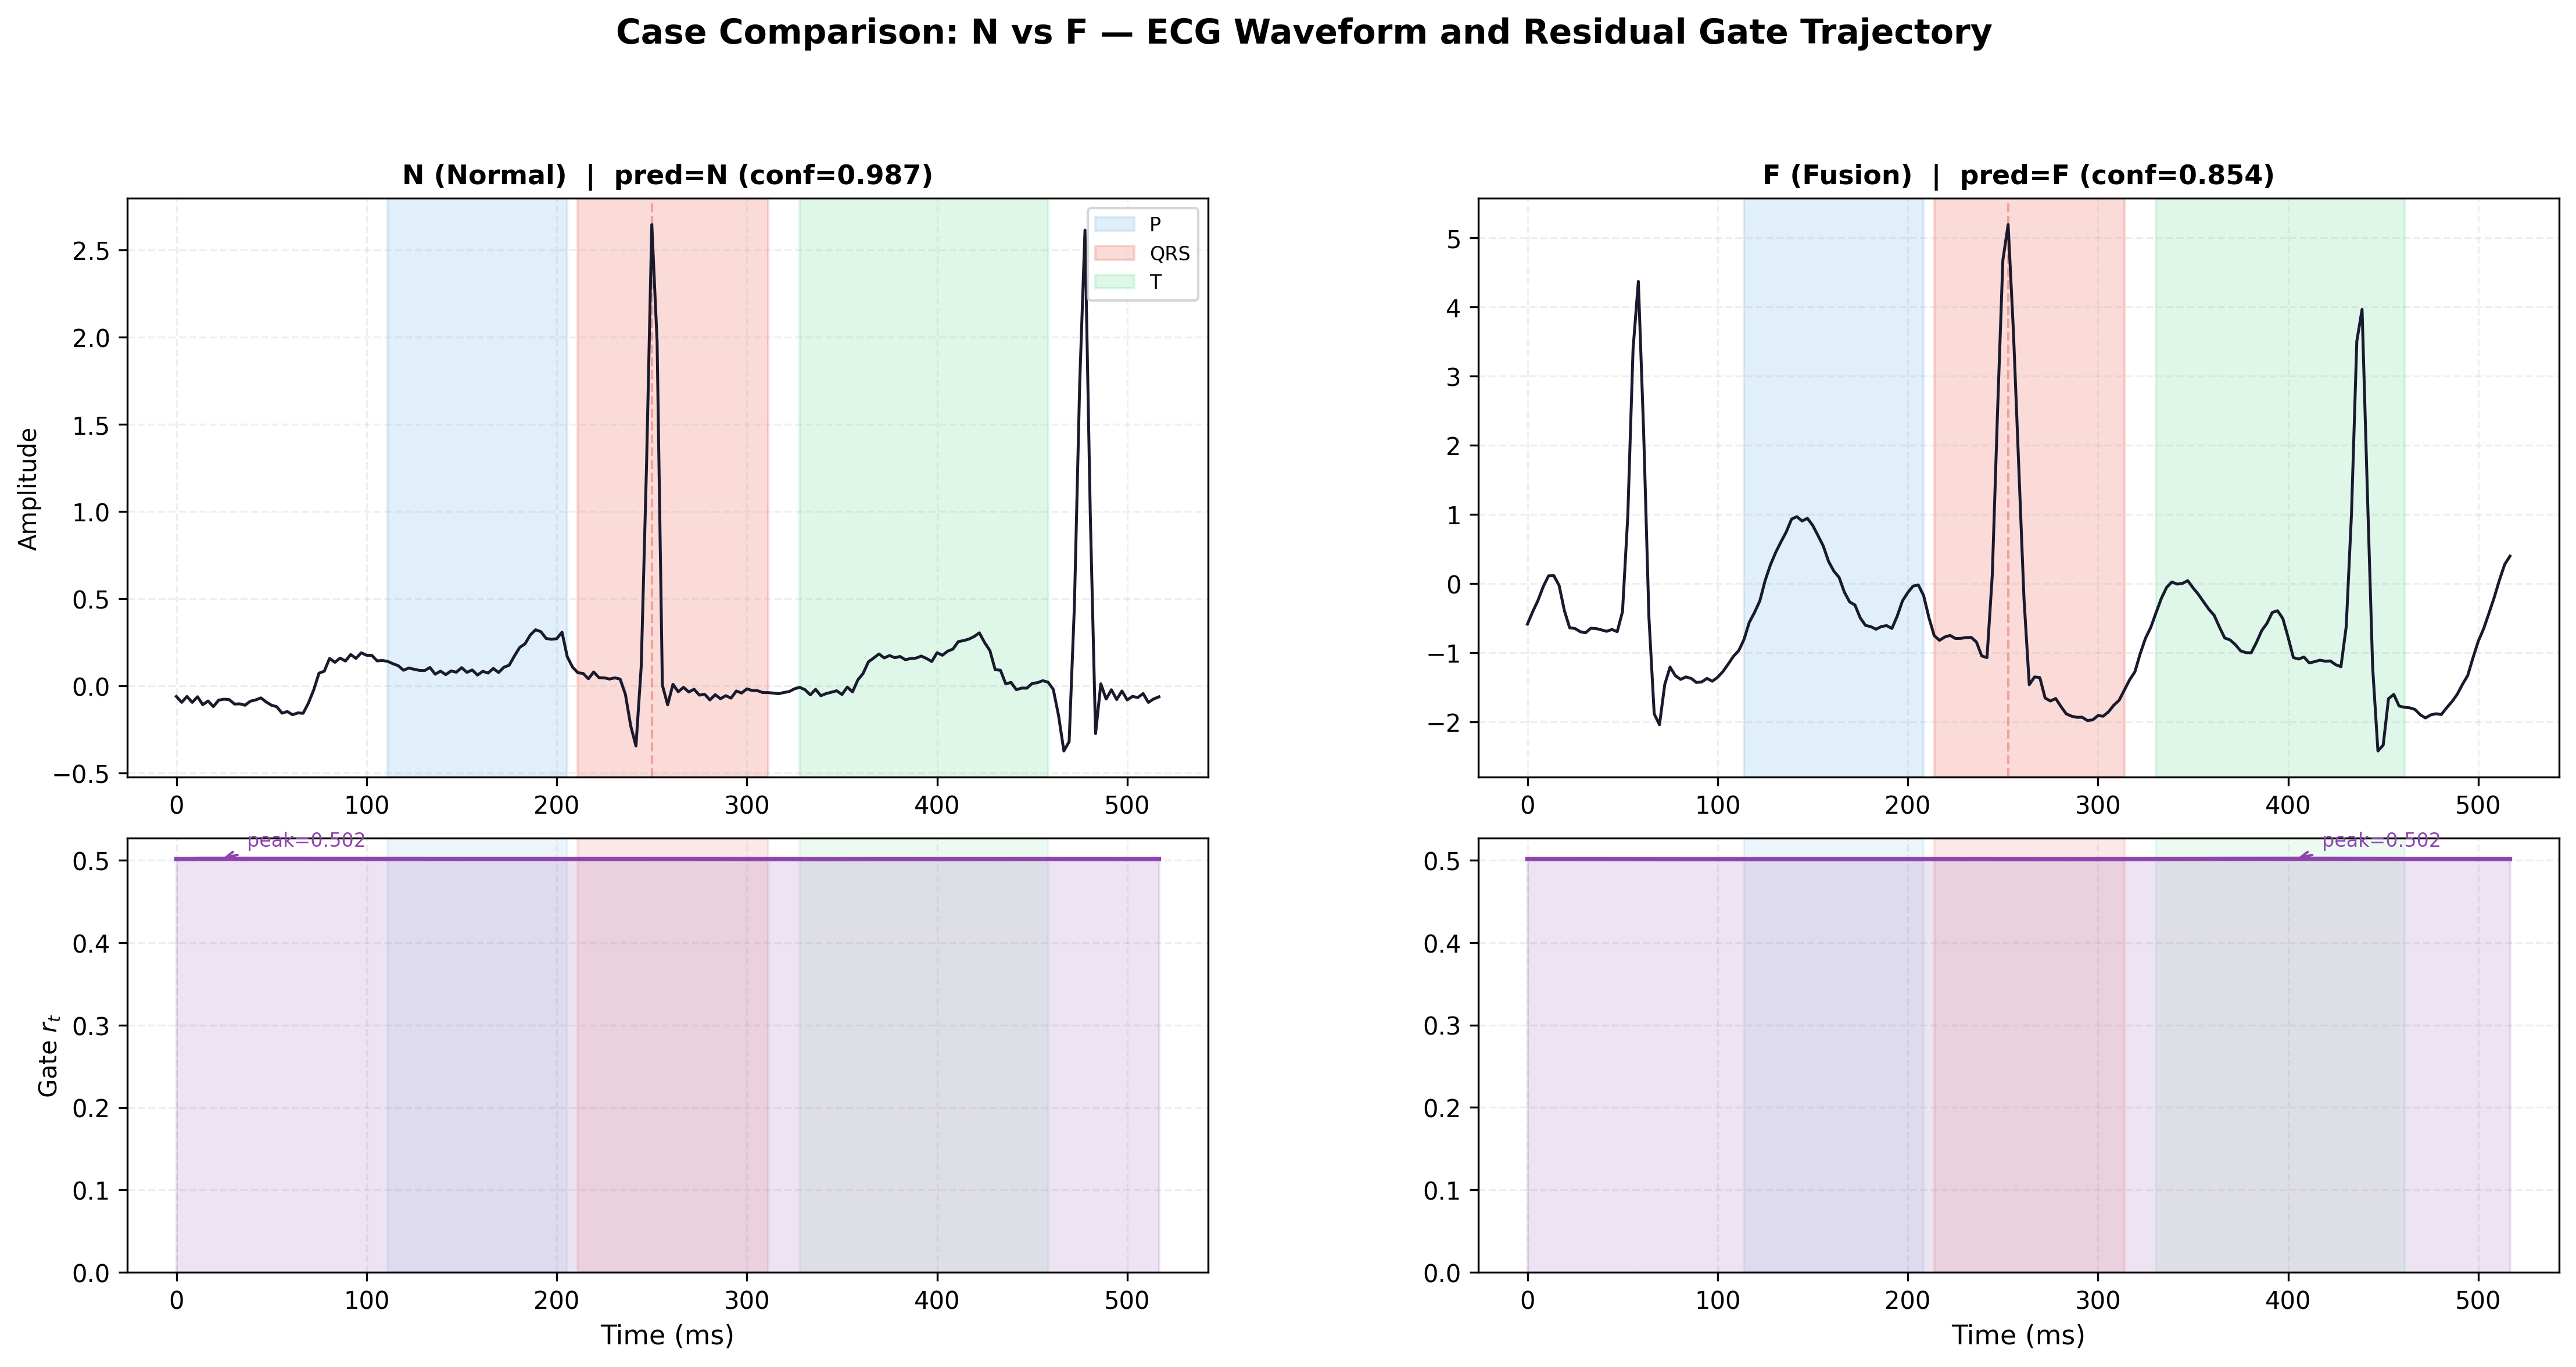
\includegraphics[width=0.8\textwidth]{images/case_comparison_N_vs_F.png}
\caption{Normal vs. Fusion case comparison (F confidence 0.8537, the lowest of the four selected cases despite being the highest-confidence correctly-classified Fusion beat available in DS2).}
\label{fig:case_f}
\end{figure}

\section{Discussion and Conclusion}
Under a strict inter-patient protocol, HMR-BiLSTM improves macro F1 by 19.1 pp and macro AUC by 12.0 pp over the strongest baseline we trained, with the improvement concentrated on -- but not fully solving -- the clinically significant Supraventricular and Fusion classes, and it degrades more gracefully than the recurrent baselines under FGSM, PGD, AutoAttack, and moderate Gaussian noise. None of this amounts to a deployment-ready claim, and we want to be explicit about why.

\textbf{Why our numbers are lower than some published MIT-BIH results.} An earlier iteration of this work, evaluated with a stratified intra-patient split (beats from the same patient could appear in both the training and test partitions), reported macro F1 of 0.8825 and AUC of 0.9916 for the same architecture family. Under the inter-patient protocol used here, the identical architecture reaches macro F1 0.6279 (canonical checkpoint) to 0.5964--0.5972 (ablation-protocol checkpoints). This is not a regression in the model; it is the expected, well-documented effect of removing patient-level leakage, since single-lead ECG morphology is highly patient-specific and a model can partially "recognise the patient" rather than the arrhythmia when beats from that patient appear in training. We verified this is not a code defect in our own pipeline (Table~\ref{tab:performance} baselines were trained and evaluated with the identical inter-patient split and show the same macro-F1 compression), and we caution readers evaluating other MIT-BIH papers to check whether a reported macro F1 above roughly 0.7--0.75 is genuinely inter-patient, was computed before or after any oversampling/SMOTE step relative to the train/test split, and reports more than top-1 accuracy, before treating it as a directly comparable number.

\textbf{Practical and societal impact.} At its current performance level, the model is best used as a triage aid on Holter monitors and wearables, flagging suspicious minority-class beats for human review rather than acting autonomously, and the uncertainty-quantification results in Section 5.6 give a concrete mechanism for that triage (route high-entropy predictions for review) that is better-behaved than relying on raw softmax confidence. Realising this depends on responsible deployment: our DS1/DS2 gains do not establish readiness across populations or devices, so prospective validation on diverse patient groups and privacy-preserving training (federated learning, differential privacy) remain prerequisites.

\textbf{Limitations.} (1) Supraventricular and especially Fusion-class performance remain well below the Normal/Ventricular classes and below credible literature benchmarks for these two classes; in follow-up experiments (reported separately) we found that patient-relative RR-interval features robustly improve Supraventricular F1 across multiple random seeds, but every configuration we tried that pushed Supraventricular detection harder simultaneously degraded Fusion-class F1, consistent with Fusion being a genuine morphological blend of Normal and Ventricular beats competing for the same decision boundary rather than an independent class that more data alone can fix; we view boundary-aware or hierarchical modelling of the Fusion class as a more promising direction than further class-weight or oversampling tuning, and leave it for future work. (2) The ablation study (Table~\ref{tab:ablation}) is single-seed; two components (the interaction term and the smoothness penalty) show an inconclusive or slightly negative measured contribution in this run that we do not consider resolved without a multi-seed re-run. (3) Calibration is good on average but poor specifically on the Supraventricular and Fusion classes (Section 5.5), and out-of-distribution detection is only weakly above chance (Section 5.6); neither should be treated as solved. (4) The AutoAttack comparison (Table~\ref{tab:autoattack}) uses a reduced 2-attack ensemble (APGD-CE + Square, fewer restarts/iterations/queries than the standard 4-attack ensemble) and a smaller 71-sample subset, for compute-budget reasons specific to HMR-BiLSTM's hand-rolled recurrent cell; the "no gradient masking" finding from this comparison should be treated as a preliminary, modest-power check rather than the full-strength AutoAttack evaluation the literature typically expects. (5) All results are single-institution, single-lead MIT-BIH; cross-dataset and cross-lead validation remain future work, as does formal clinician review of the interpretability outputs in Section 5.7.

\section*{Acknowledgement}
This research is funded by the University of Economics Ho Chi Minh City, Vietnam (UEH).

\section*{Data Availability}
The ECG datasets used in this study are publicly available from the MIT-BIH Arrhythmia Database (PhysioNet). The implementation code, experimental configurations, and evaluation results are available at: \url{https://github.com/Lamno1/HMR-BiLSTM-Trustworthy}


\setlength{\bibsep}{0pt}
\bibliography{mau1}

\end{document}
